We start the research of the presence of cycle-by-cycle sequential restrictions found in \textcite{elices_robust_2019} by exploring them in a computational model. The detailed reproduction of the activity allows to study in detail the mechanisms associated to the circuit and the time-interals relations. We used the feeding CPG model description of \textcite{vavoulis_dynamic_2007}, which even though it does not have a chaotic mode, the model is flexible enough to adapt the variability of one of the neurons. Following the current injection protocol defined in section \ref{subsec:inj protocol}, N1M, N3t and SO neurons in the model were stimulated for our analysis of the sequence interval variability. Using this induced variability we were able to explore the presence of sequential dynamical invariants under different scenarios. The effect on injecting a current ramp on N2v is not reported here since it leads to lower variability than the other cases. In all simulations, we could test the robustness of the rhythm while inducing the external perturbation that evoked variability in the search for dynamical invariants. The results summarized and adapted for this section were published in \cite{garrido-pena_characterization_2021}.

First we saw that the model of the feeding CPG faithfully reproduces the activity of the main neurons involved in the generation of its triphasic rhythm \parencite{vavoulis_dynamic_2007}. This includes their waveforms and the relationships between the cycle period and the duration of several intervals reported in \parencite{elliott_temporal_1991}. Note that, since there was not a description of a chaotic mode, all the rhythms explored here were analyzed from induced stimulation, not by simulating spontaneous activity. This was a restriction when exploring spontaneous activity, since the circuit needed to be altered by one of the neurons, simulating a extended experimental protocol, but still altering the circuit in a predefined way. Also, other phenomena reported in the pyloric CPG experimental work, were there was a "reset" in the inter-cycle dynamics of the dynamical invariants, could not be explored in this model, since the ramp value was progressive (see Apendix Fig. \ref{fig:N1M stimulation pairplot reset} for a representation of this non-reset output). All this will be illustrated in the following Section \ref{sec:experimental sussex} with experimental recordings and other options to reproduce the functional variability will be discussed in Section \ref{sec:model variability}.

\subsection{N1M driven variability}
\label{subsec:n1m driven}

N1M neuron can be stimulated using ramp protocols in living preparations \parencite{elliott_temporal_1991} as it plays an important role in initiating the CPG rhythm. In our case, after applying the current injection protocol into N1M and detecting the spike and burst events for each neuron in the CPG model, all  intervals represented in Fig. \ref{fig:intervals} were quantified. We show in Fig. \ref{fig:invariant n1m} the variability and the correlation between the period and each interval.

\begin{figure}[hbt!]
	\begin{minipage}[b]{0.45\textwidth}
		\centering
		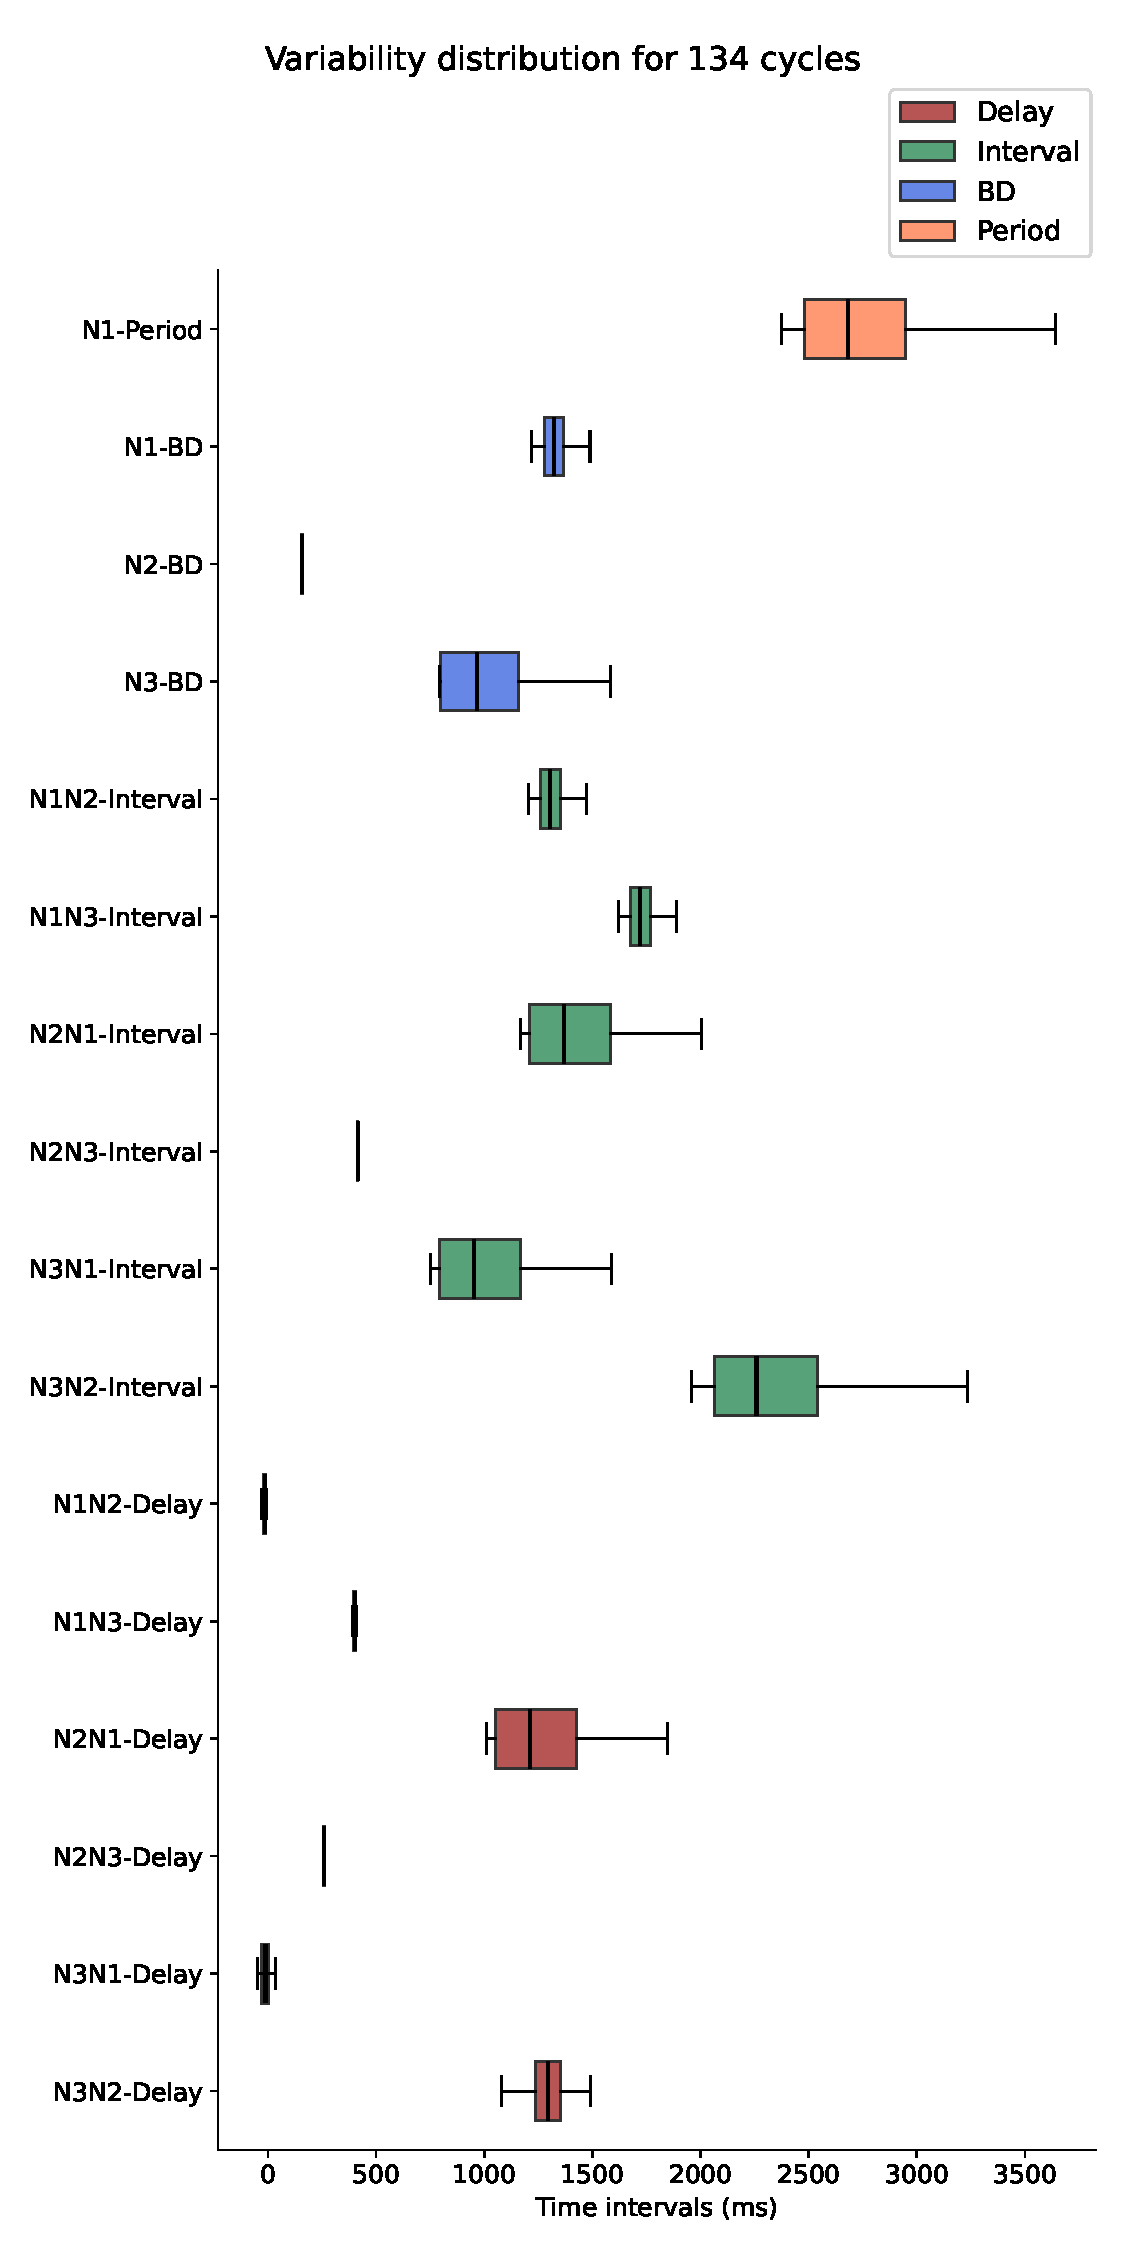
\includegraphics[width=\textwidth]{invariants/data/MODEL/n1m_driven/images/3phases/_boxplot.pdf}
	\end{minipage}
	\begin{minipage}[b]{0.53\textwidth}
		\centering
		\begin{minipage}[b]{\textwidth}
			\centering
			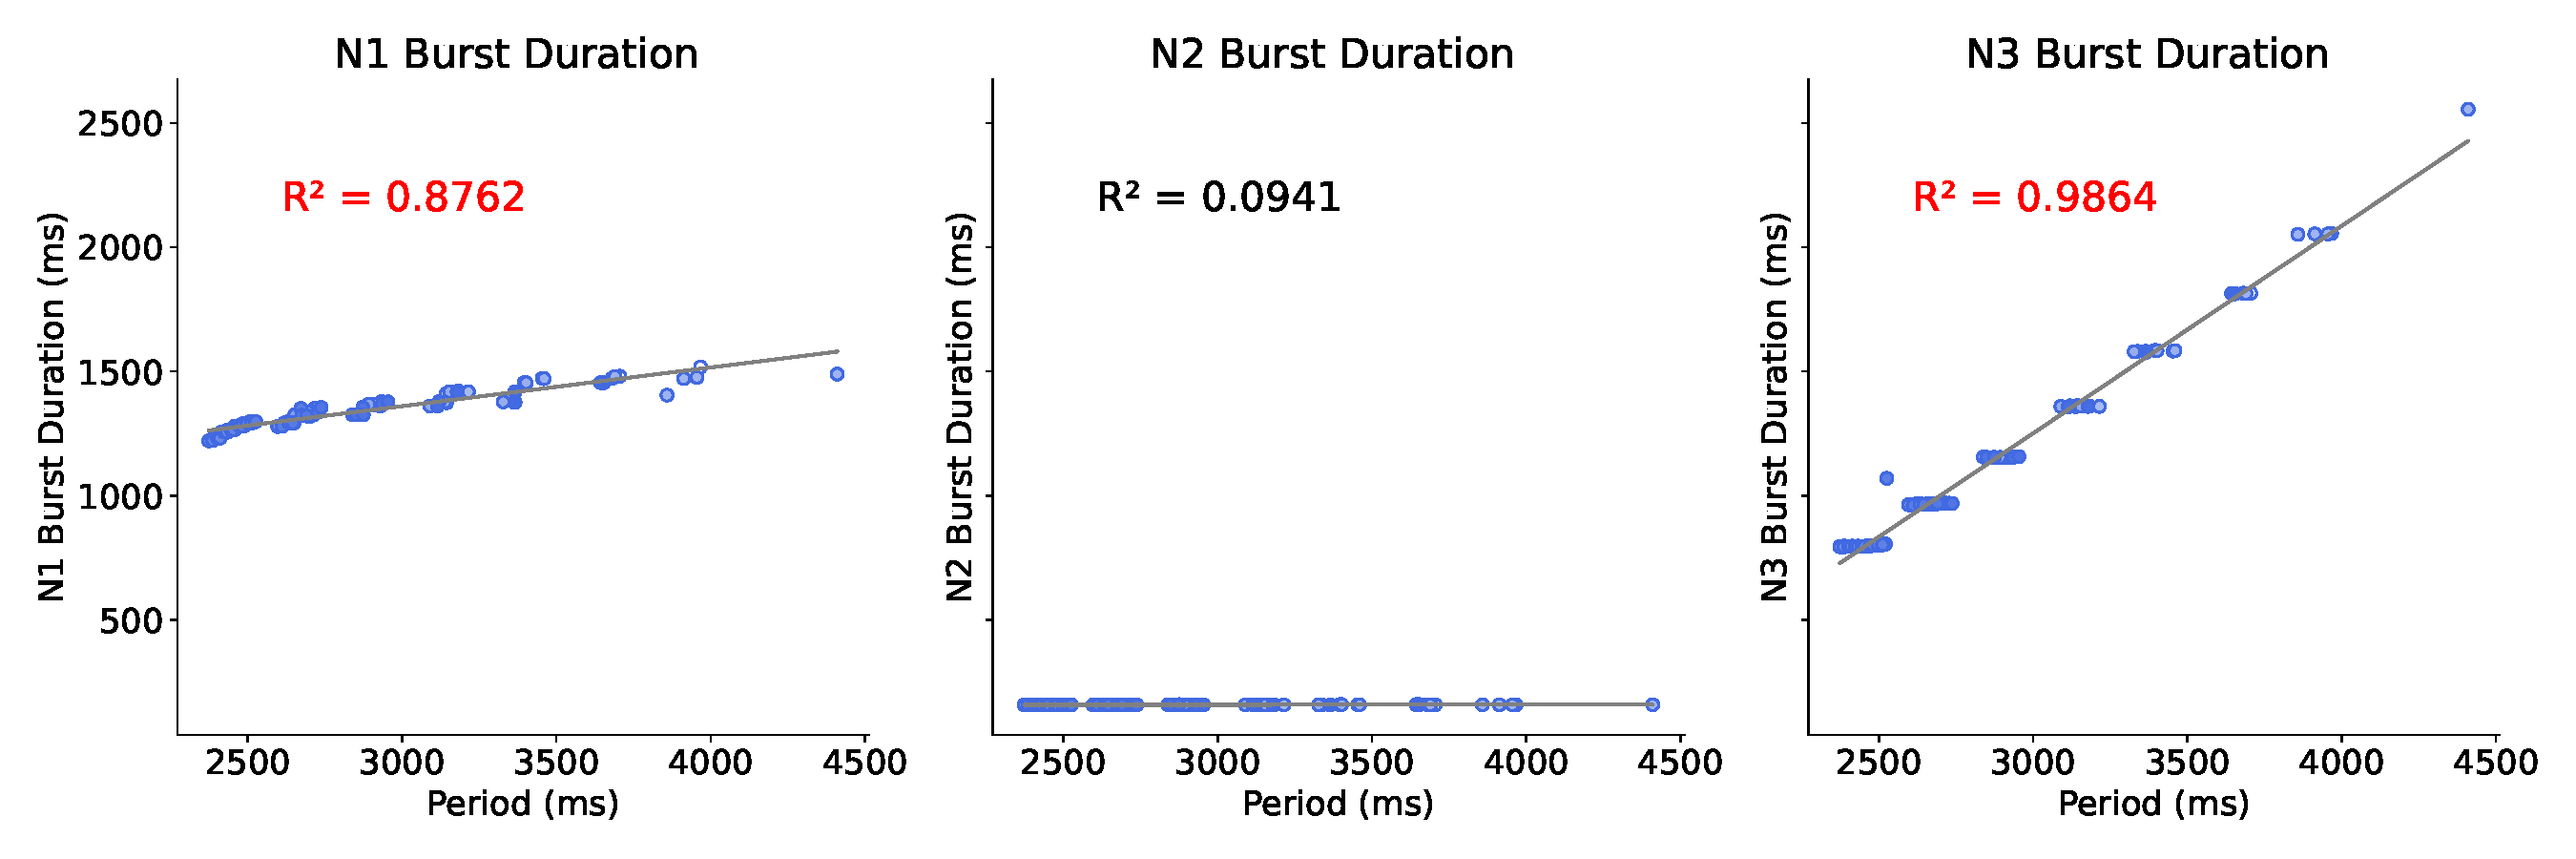
\includegraphics[width=\textwidth]{invariants/data/MODEL/n1m_driven/images/3phases/_durations.pdf}
		\end{minipage}\
		\begin{minipage}[b]{\textwidth}
			\centering
			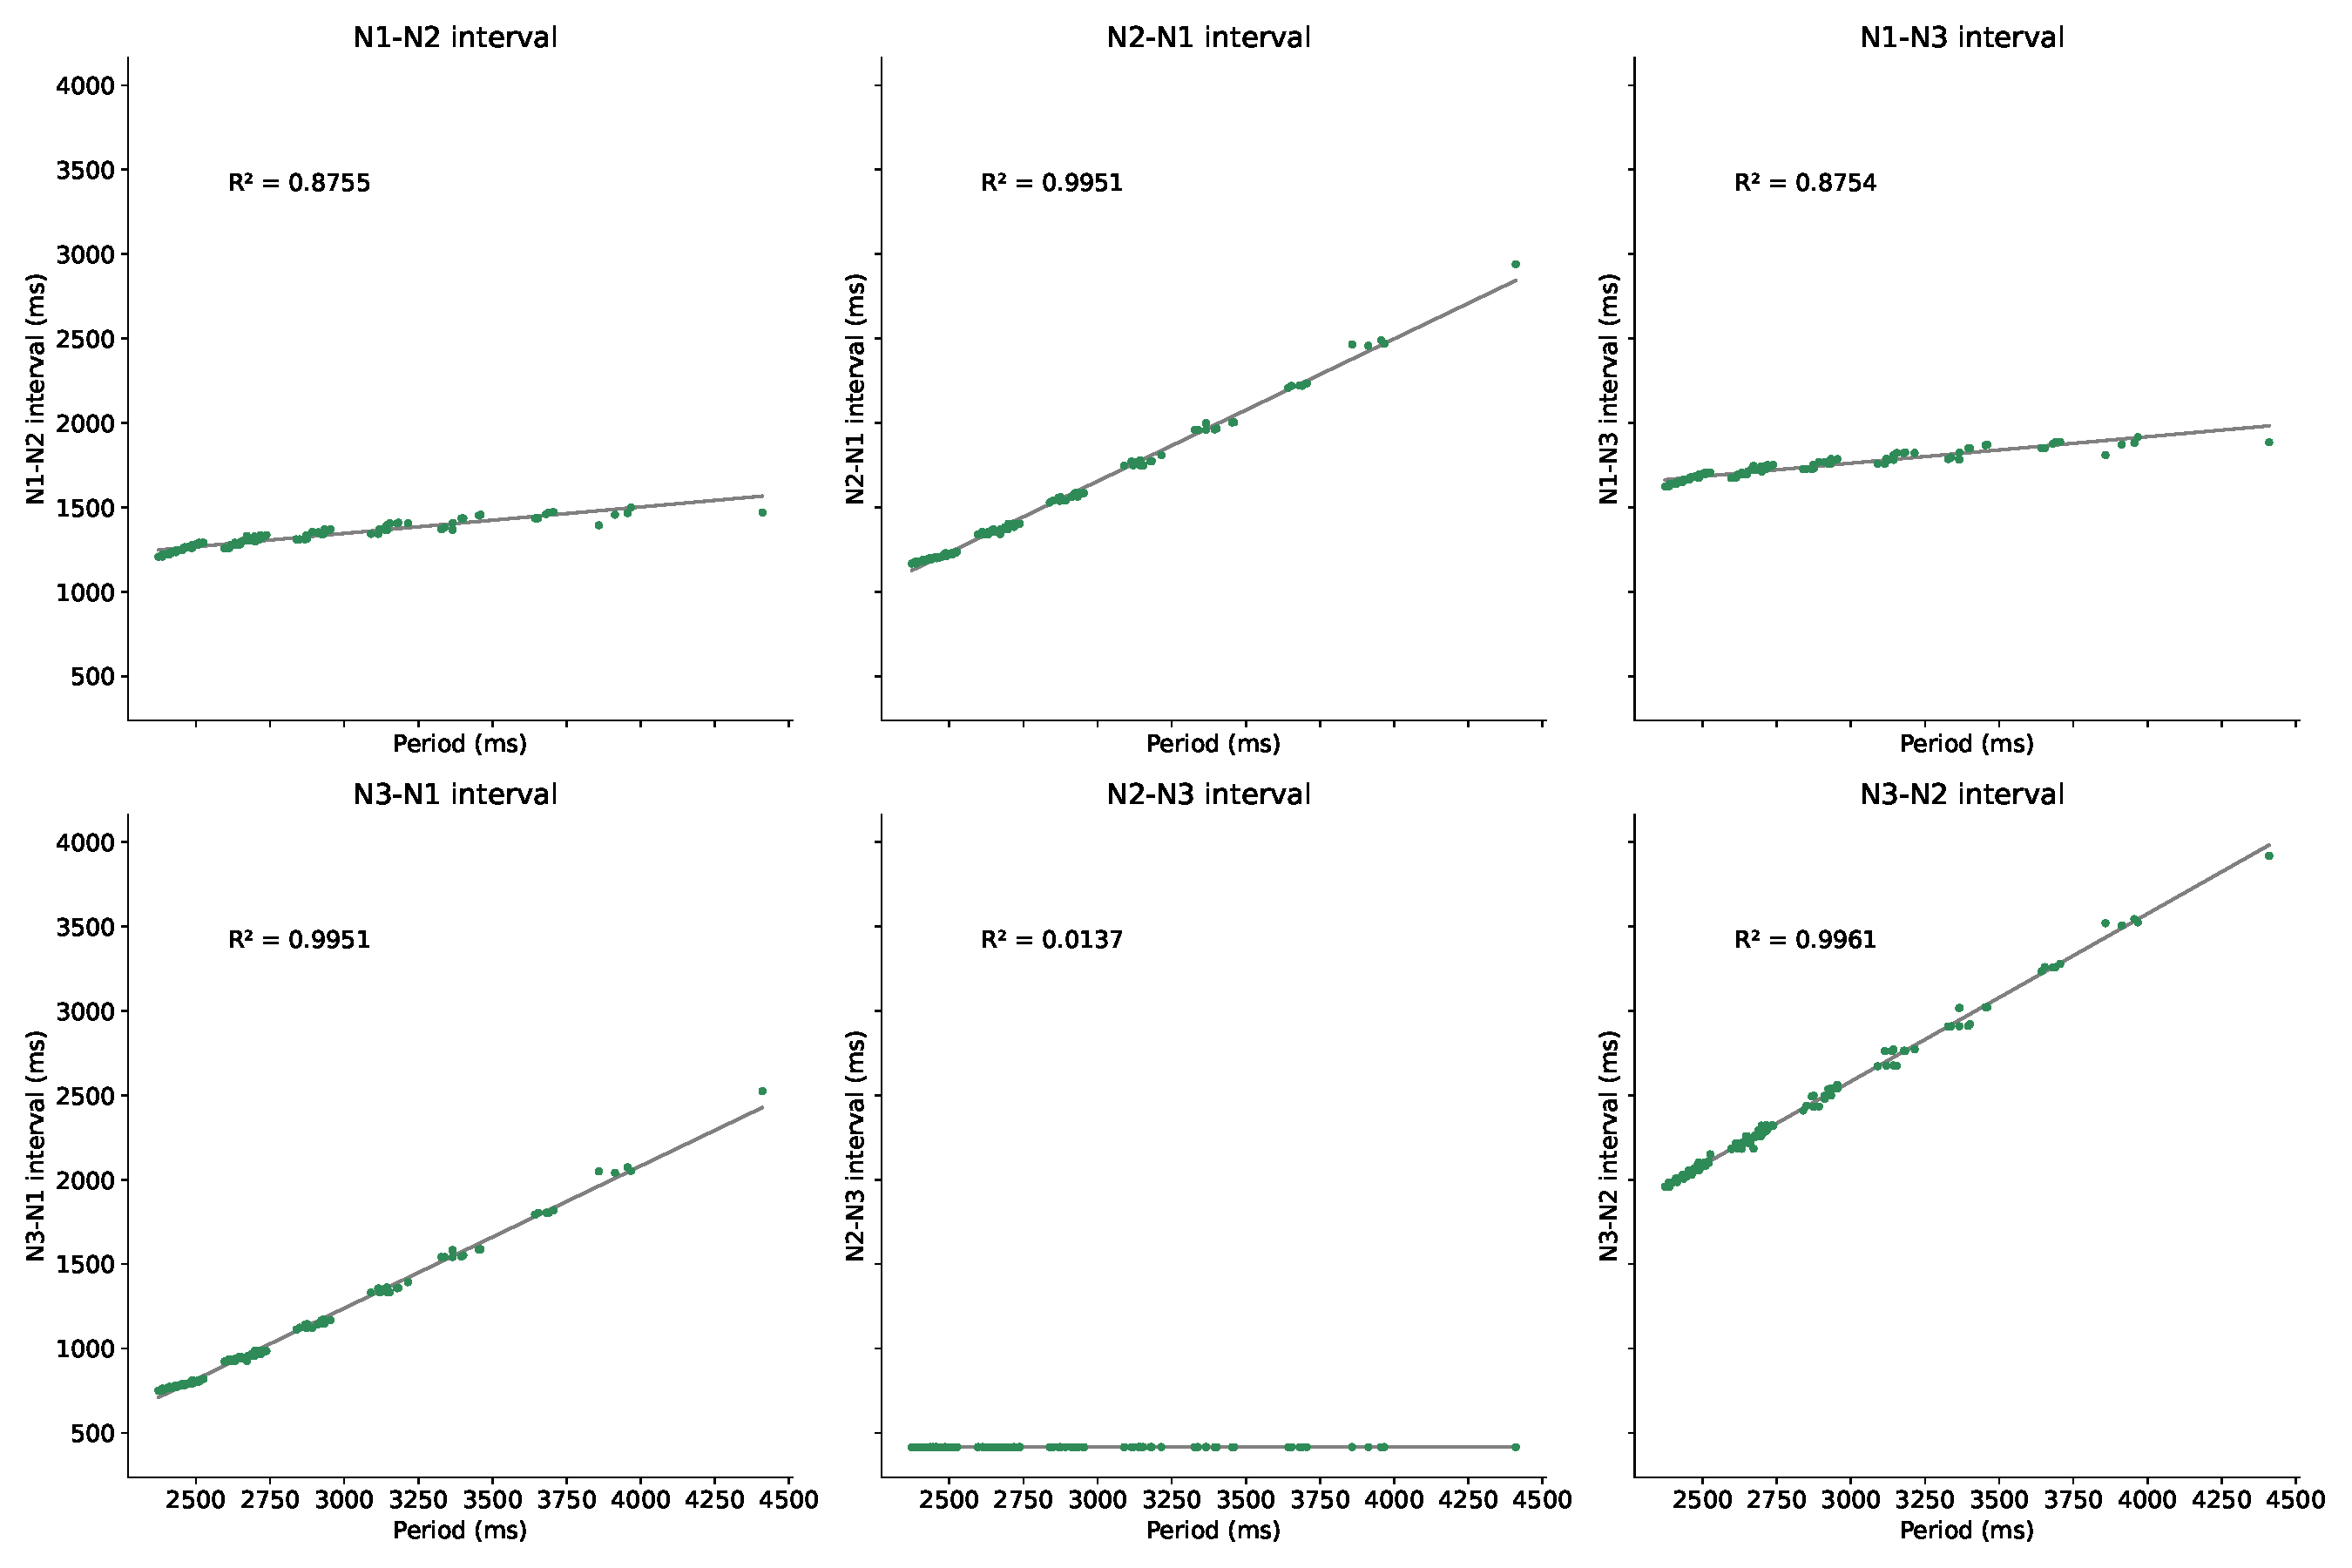
\includegraphics[width=\textwidth]{invariants/data/MODEL/n1m_driven/images/3phases/_intervals.pdf}
		\end{minipage}\
		\begin{minipage}[b]{\textwidth}
			\centering
			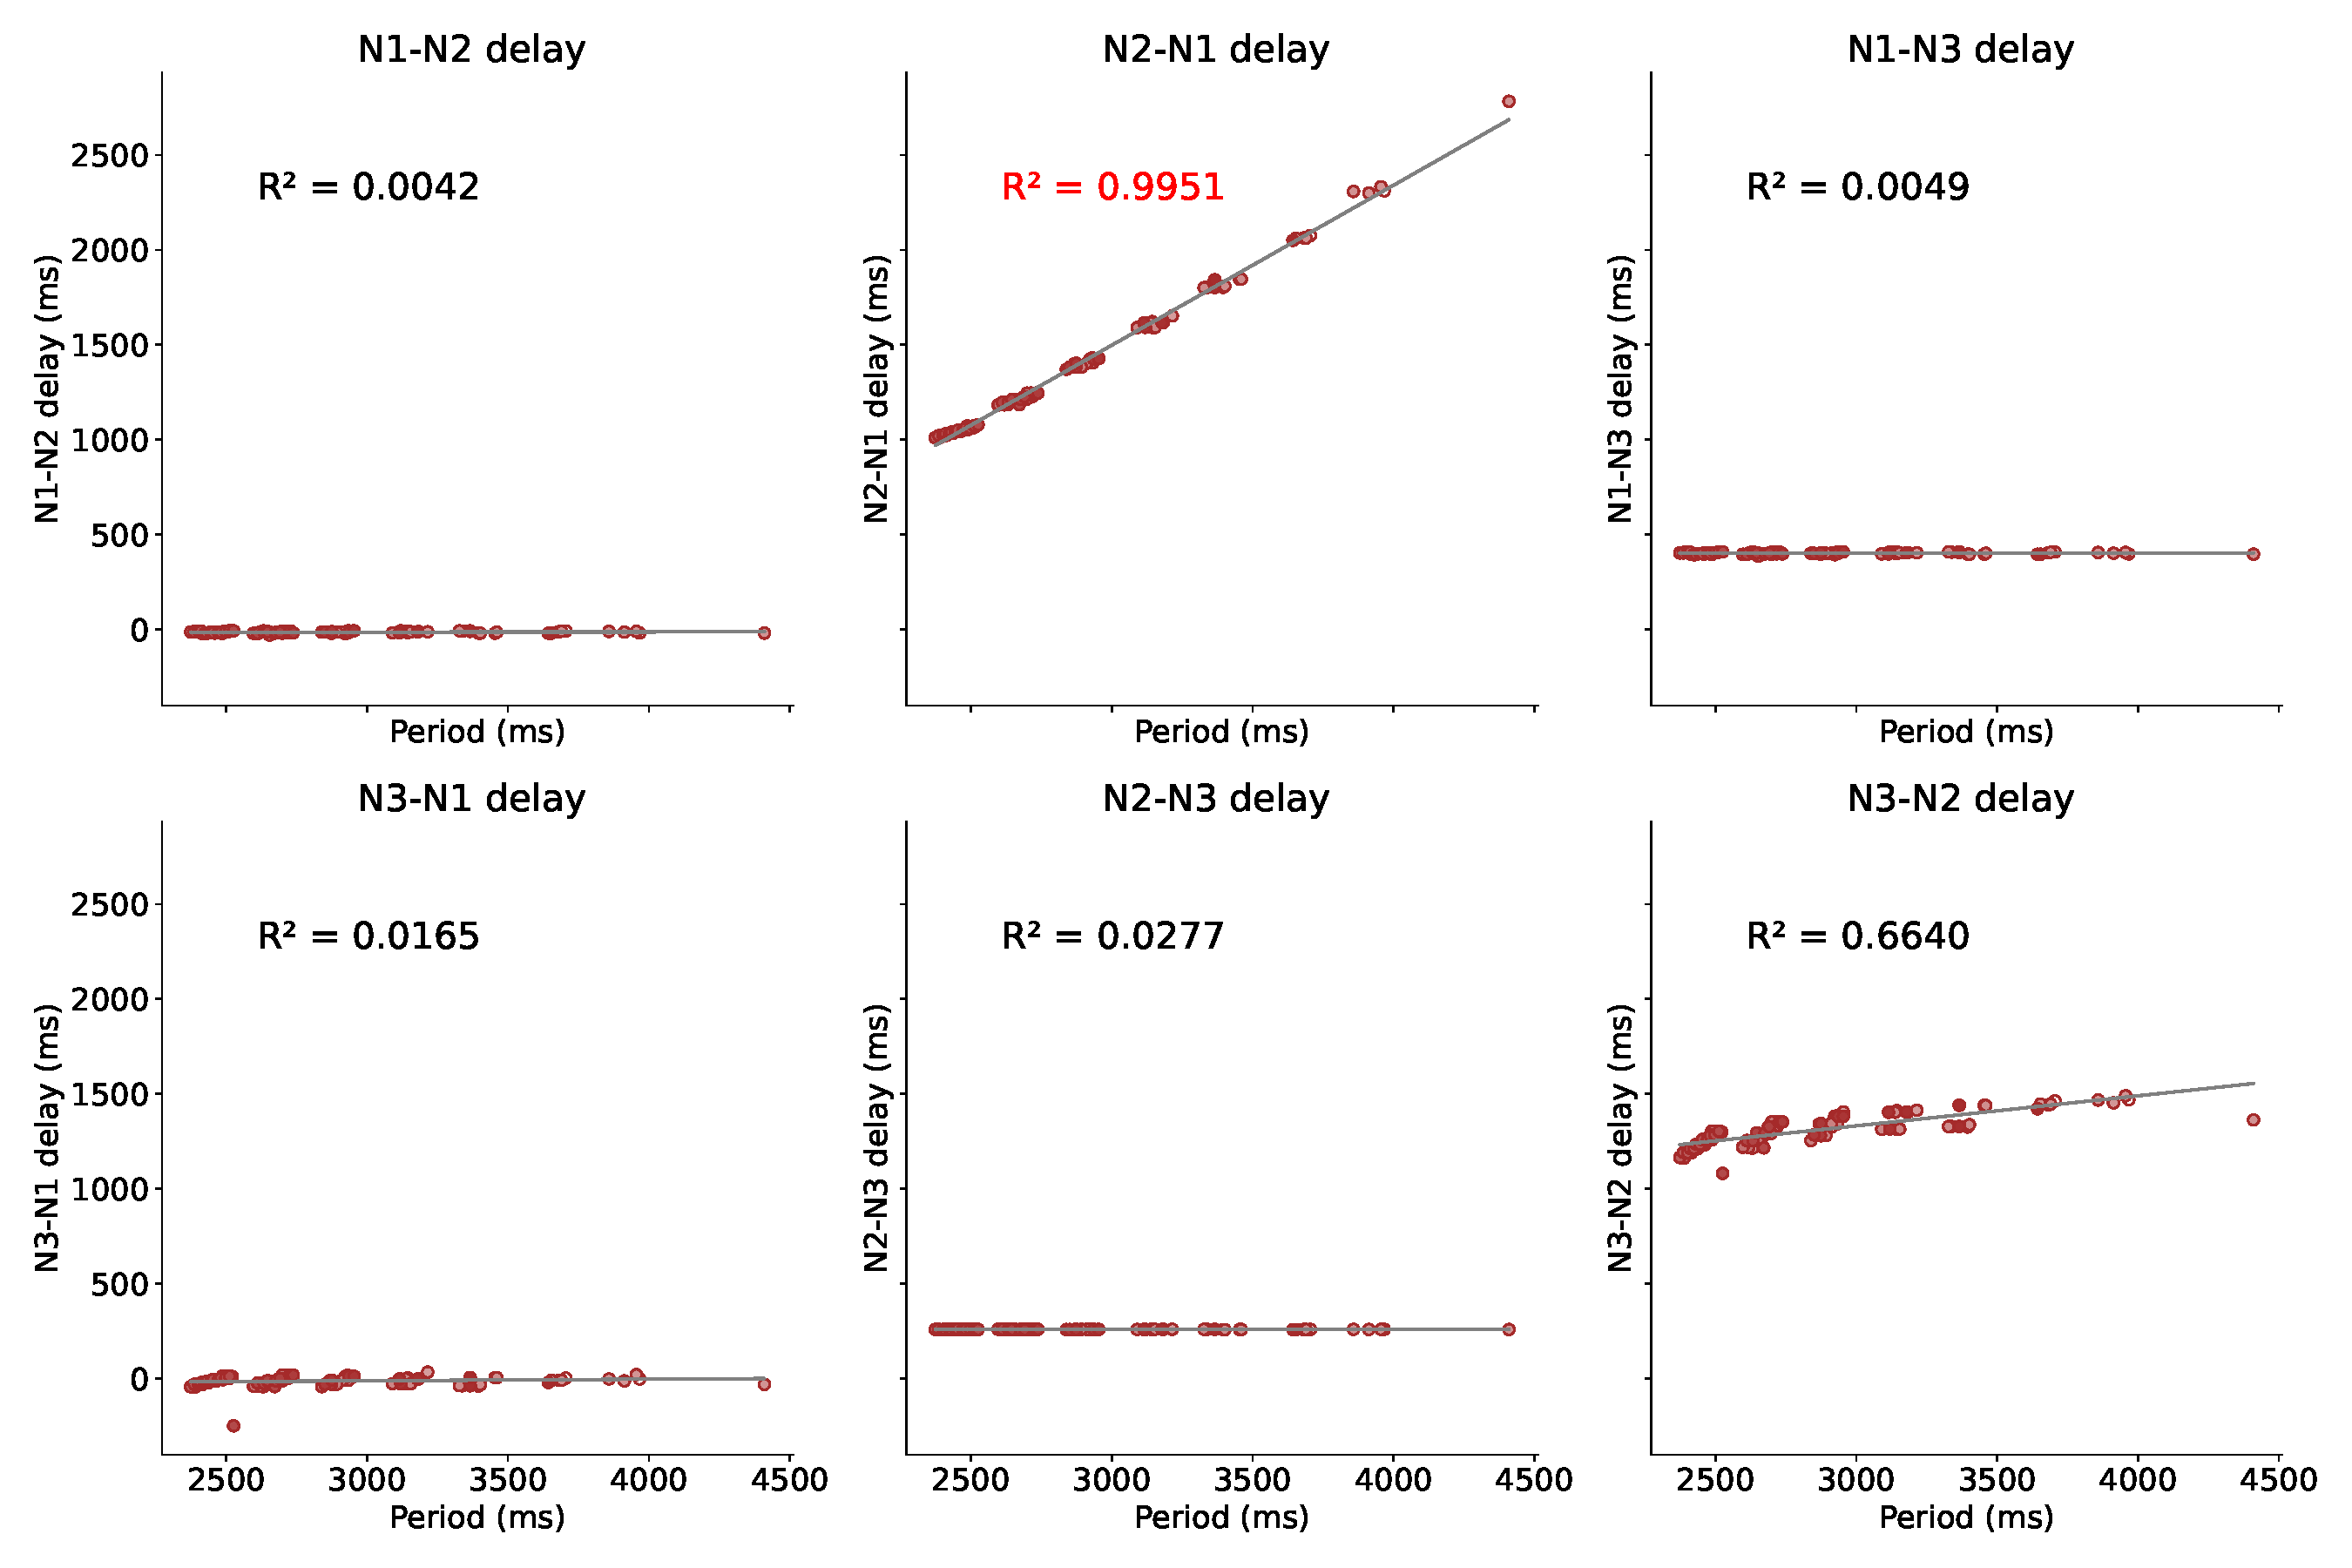
\includegraphics[width=\textwidth]{invariants/data/MODEL/n1m_driven/images/3phases/_delays.pdf}
		\end{minipage}
	\end{minipage}
	\caption{\textbf{N1M stimulation:} a) Box-plots of the  sequence intervals under N1M neuron stimulation. b) Interval correlations to period for N1M-driven simulation. First row: Burst duration. Second and third row: Two-neuron intervals. Forth and fifth row: Two-neuron delays. Linear relationships are quantified by the $R^2$ values of the linear regression.}
	\label{fig:invariant n1m}
\end{figure}

Figure \ref{fig:invariant n1m}.a) displays the boxplots of the duration of all sequence intervals defined above. Regarding burst duration of the neurons (N1M-BD, N2v-BD, N3t-BD), we can observe in this figure that the most variable one corresponds to N3t neuron. Furthermore, the derived intervals which cover N3 phase are also the ones presenting larger variability (i.e., N2-N1, N3-N1 and N3-N2 intervals and N2-N1 delay). On the other hand, the least variable intervals correspond to the ones related to N2v and N1M burst duration, i.e., N1-N2, N1-N3, N2-N3 intervals and N1-N2, N1-N3, N3-N1, N2-N3, N3-N2 delays. They show a nearly a constant duration during each period.

Figure \ref{fig:invariant n1m}.b) plots the cycle-by-cycle measurements of the intervals defined in \ref{fig:intervals} against the period. The first row displays burst duration intervals, which are the intervals analyzed in \textcite{elliott_temporal_1991} from data obtained in electrophysiological recordings of living neurons, and in Vavoulis et al. from data obtained in model simulations \parencite{vavoulis_dynamic_2007}. The results shown in this row match those results, being N3t-BD the most correlated to the period, which can be noted by the $R^2$ value close to one in the linear regression. The other two intervals (N1M-BD and N2v-BD), which were also the least variable, are not strongly correlated to the period. For our discussion in this case and the following cases reported here, we focus on invariant relations with R2>0.9 and large slopes in the resulting linear regression to the data. 

Likewise, the most variable intervals derived from other time references of the sequence also show a high correlation with the period, i.e., they present dynamical invariants, in this case N2-N1, N3-N1, N3-N2 intervals and N2-N1 delay. The cycle-by-cycle period variability is a consequence of the variability in these specific intervals.

On the other hand, intervals related to neuron N2v and N1M are the least variable. N2v is the one least affected by the global activity of the circuit, in terms of its burst duration. Moreover, some of the intervals are very short, or even negative, since the end of a given neuron's burst overlaps the next one's beginning (N1-N2 and N3-N1 delay). This is the case for N1-N2 and N3-N1 delay (4th row, 1st column and 5th row, 1st column, respectively in Fig. \ref{fig:invariant n1m}.b).  




\subsection{N3t driven variability}
\label{subsec:n3t driven}

The stimulation protocol was also applied to N3t neuron. Although no previous analysis on injecting a current ramp into this neuron has been reported neither experimentally nor in the feeding CPG computational model, due to the connectivity in the circuit, it can be expected that the stimulation of N3t will induce variability in the rhythm. The characterization of the sequence intervals in this case are shown in Fig. 
\ref{fig:invariants n3t}.a) and the correlation analysis is displayed in Fig. \ref{fig:invariants n3t}.b).
%In fact, we can expect a similar result to N1M-driven simulation because of their bidirectional connectivity see Fig. \ref{fig:CPG diagram}.  ***dicutir si es siméterica o no *****


Results shown in Fig. \ref{fig:invariants n3t}.a) indicate that the larger variability is present in the same intervals related to N3t burst duration, as when the stimulation was delivered to N1M. However, in this simulation we observe that N1M had a lower variability while N3t had a higher variability with respect to the previous condition. 
%: N1M decreased its variability while N3t has increased it *****discutir***. 
In contrast, N2v-BD maintained its variability, as well as all the derived intervals containing this burst duration.

Note that N3-N1 delay, which is the interval from the end of the N3t burst to the beginning of N1M burst, shows negative values. This means that neuron N1M started earlier than the end of N3t in every cycle. Whilst this was also present in N1M-driven activity simulations, here the variability of this interval is much higher, leading to a larger overlapping.
% N2v maintains its variability, being this interval and all the intervals related to it the least variable. Hence, in the distribution of the activity in the circuits between the neurons, the main negotiation is between N1M and N3t, distributing the variability and the period leading between they both. ***esto también lo tenemos que pulir un poco****

Figure \ref{fig:invariants n3t}.b) plots each interval duration against the period. As in the previous condition, the dynamical invariants (i.e. intervals presenting a strong correlation to the period) show up in the intervals related to N3 phase, which were the ones presenting also the highest variability, whereas those intervals that do not participate in dynamical invariants, are the ones related to N1M and mostly N2v (the least variable ones). 


%The linear relationships regarding the least variable intervals (related to N2v and N1M burst durations), also present similar results to those discussed above when the rhythm was driven by N1M. Hence, the intervals most correlated are the ones with higher variability, whereas those intervals that do not participate in dynamical invariants, are the ones related to N1M and mostly N2v (the least variable ones).
%***revisar redundancia***


\begin{figure}[hbt!]
	\begin{minipage}[b]{0.45\textwidth}
		\centering
		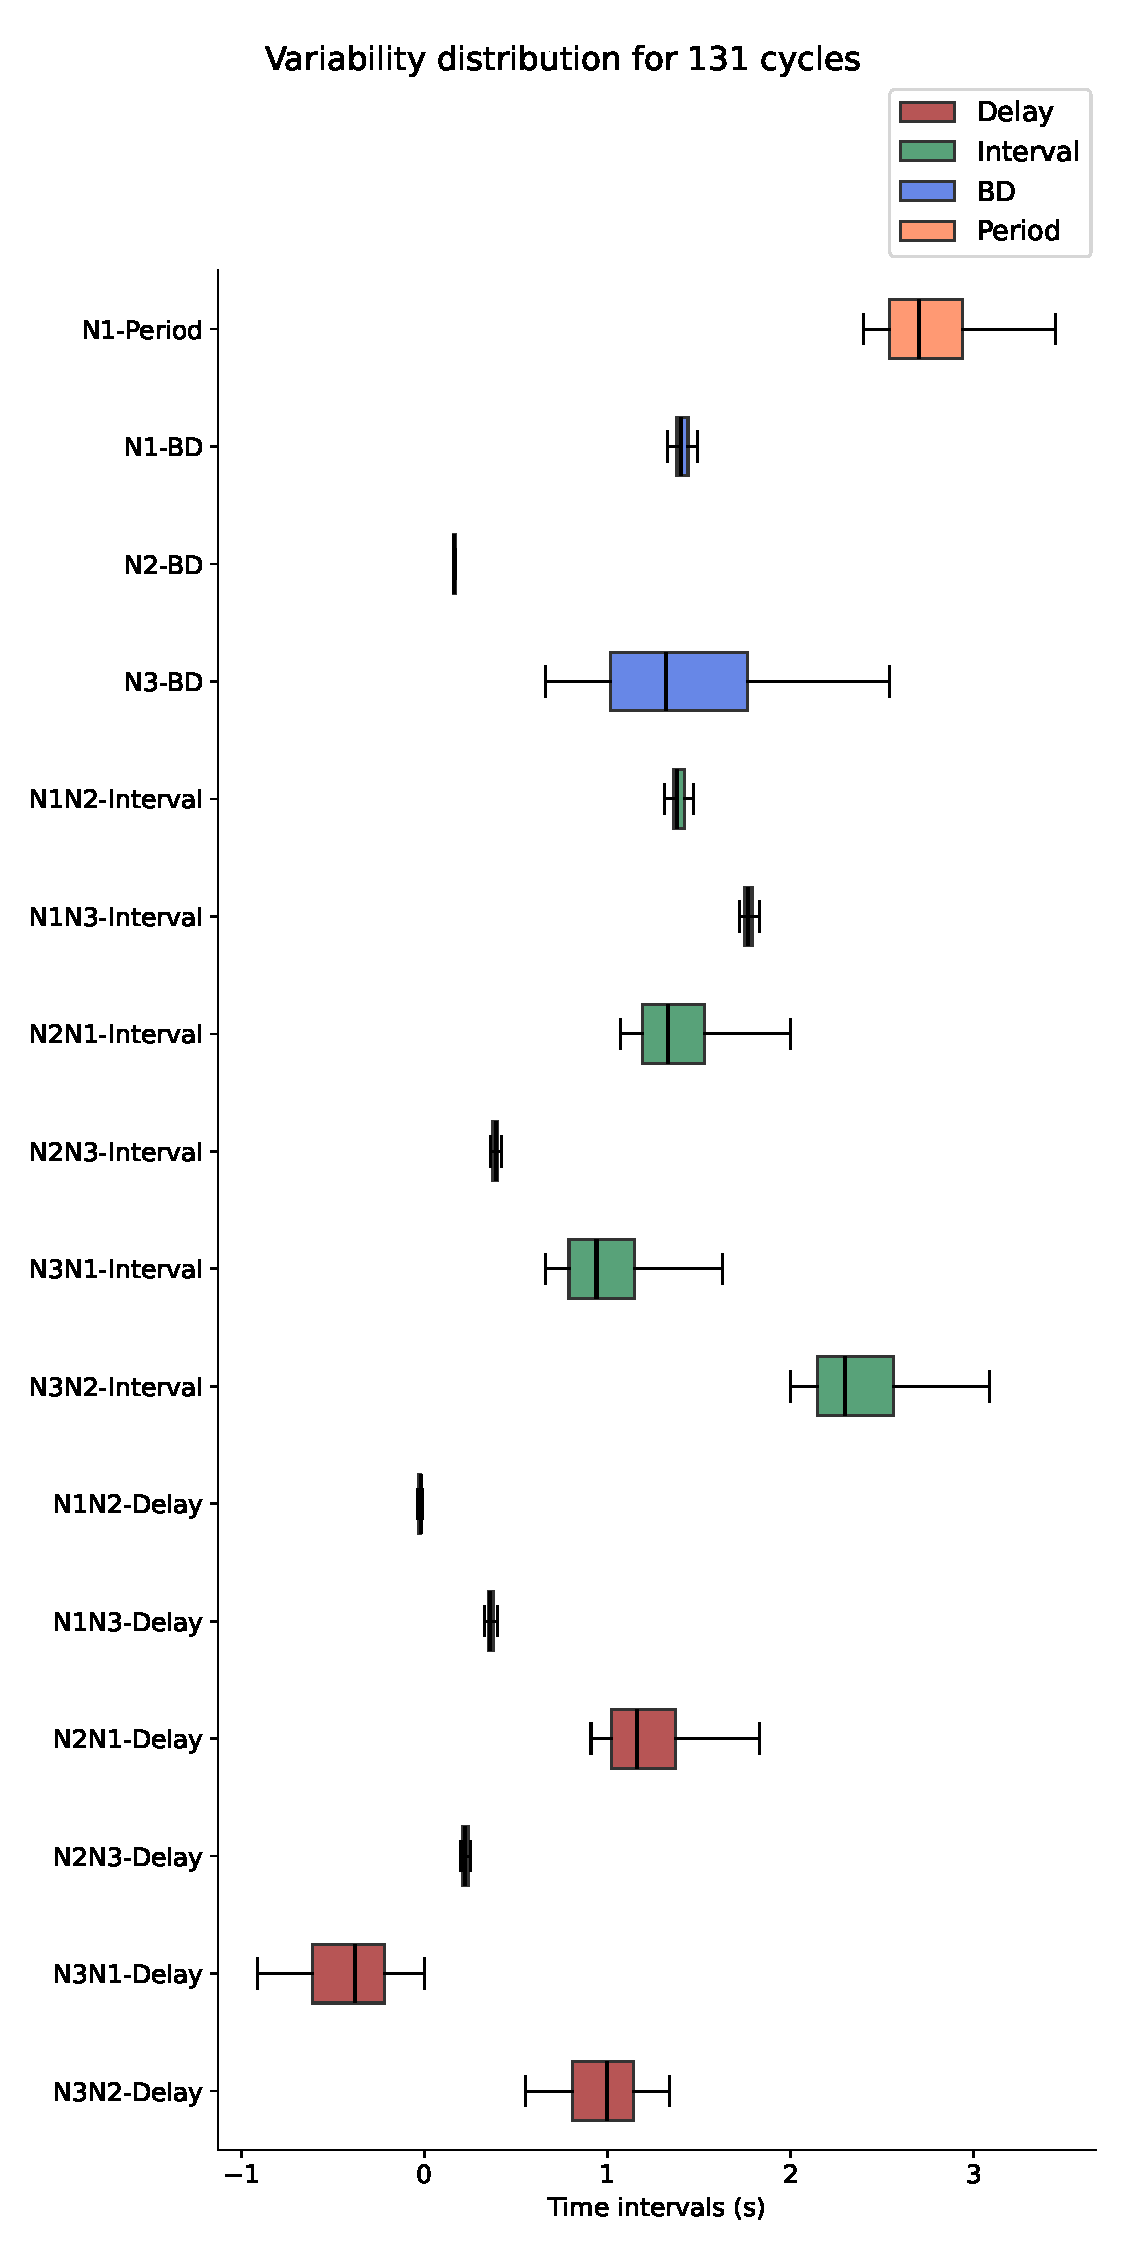
\includegraphics[width=\textwidth]{invariants/data/MODEL/n3t_driven/images/3phases/_boxplot.pdf}
	\end{minipage}
	\begin{minipage}[b]{0.53\textwidth}
		\centering
		\begin{minipage}[b]{\textwidth}
			\centering
			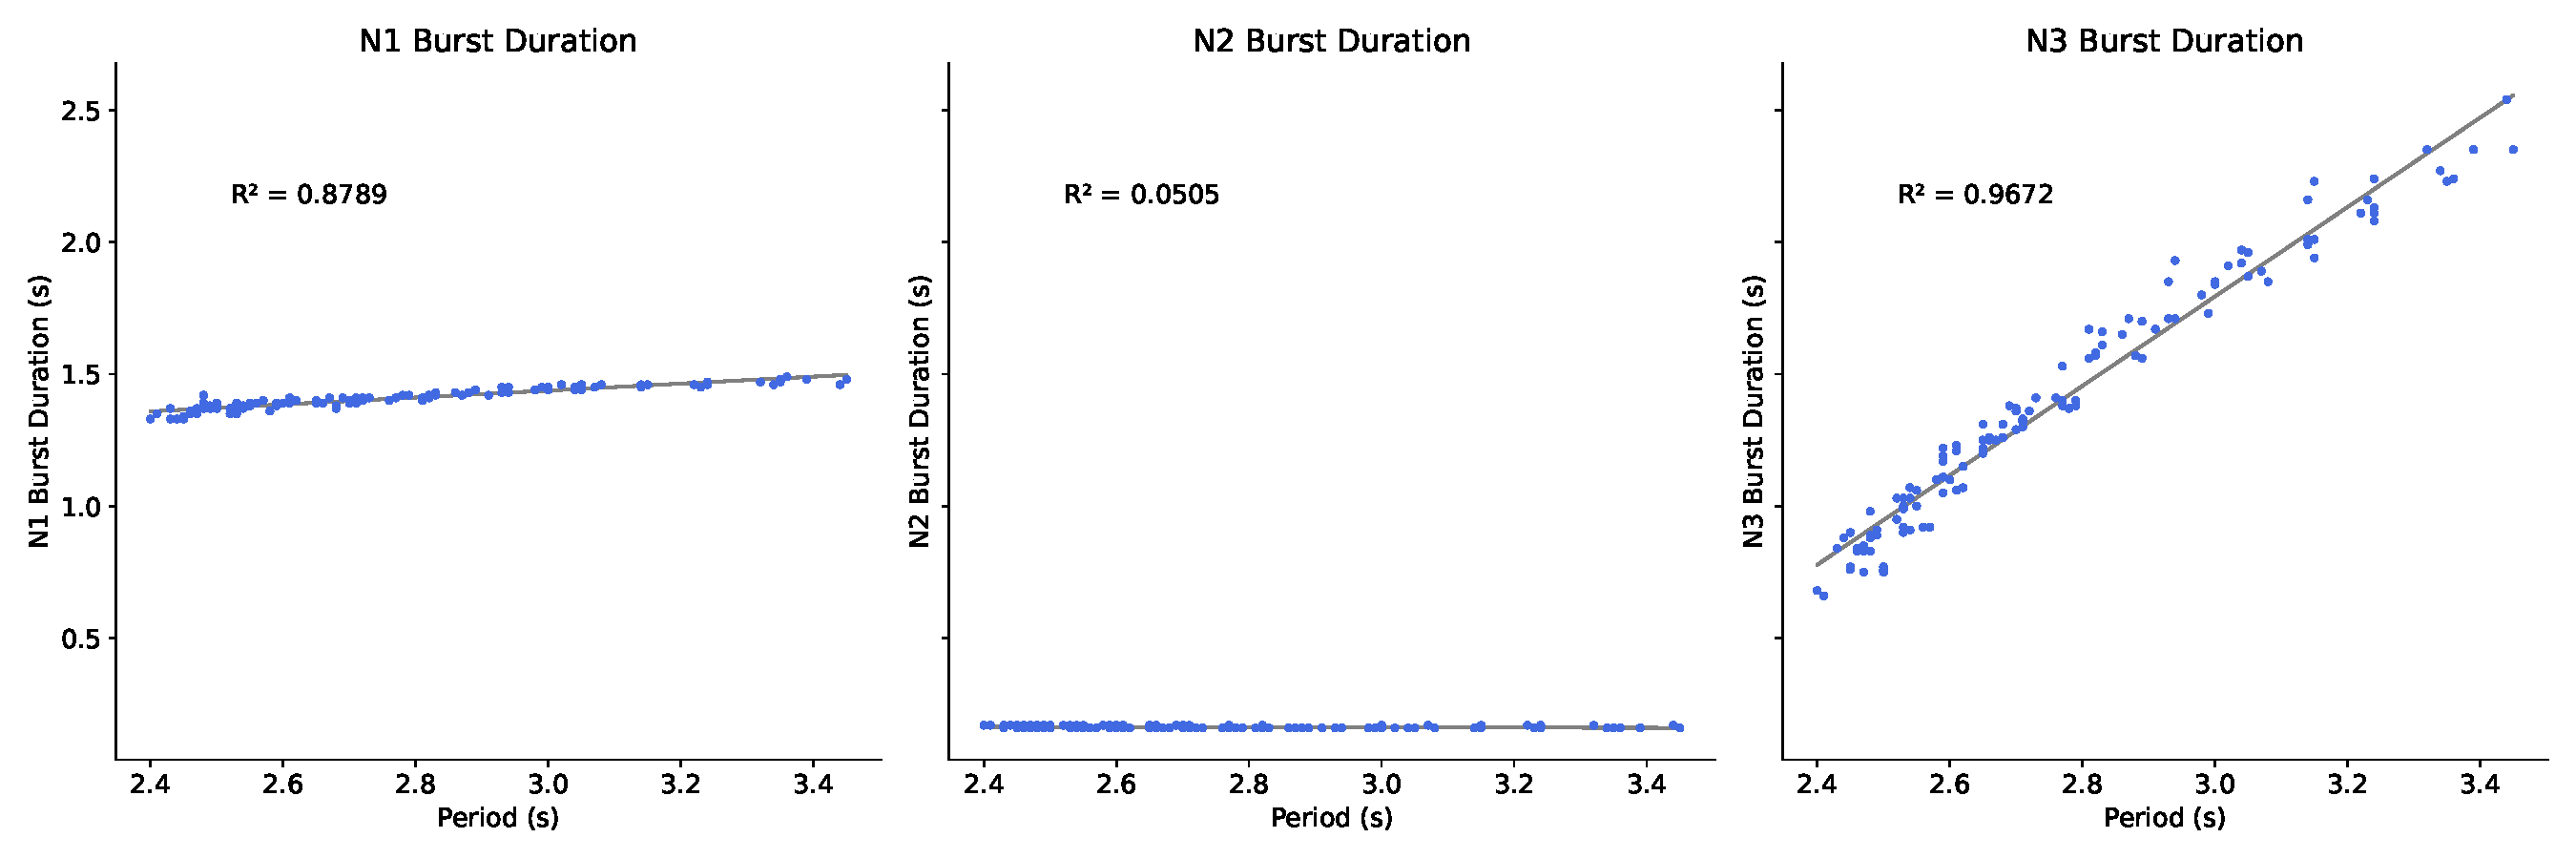
\includegraphics[width=\textwidth]{invariants/data/MODEL/n3t_driven/images/3phases/_durations.pdf}
		\end{minipage}\
		\begin{minipage}[b]{\textwidth}
			\centering
			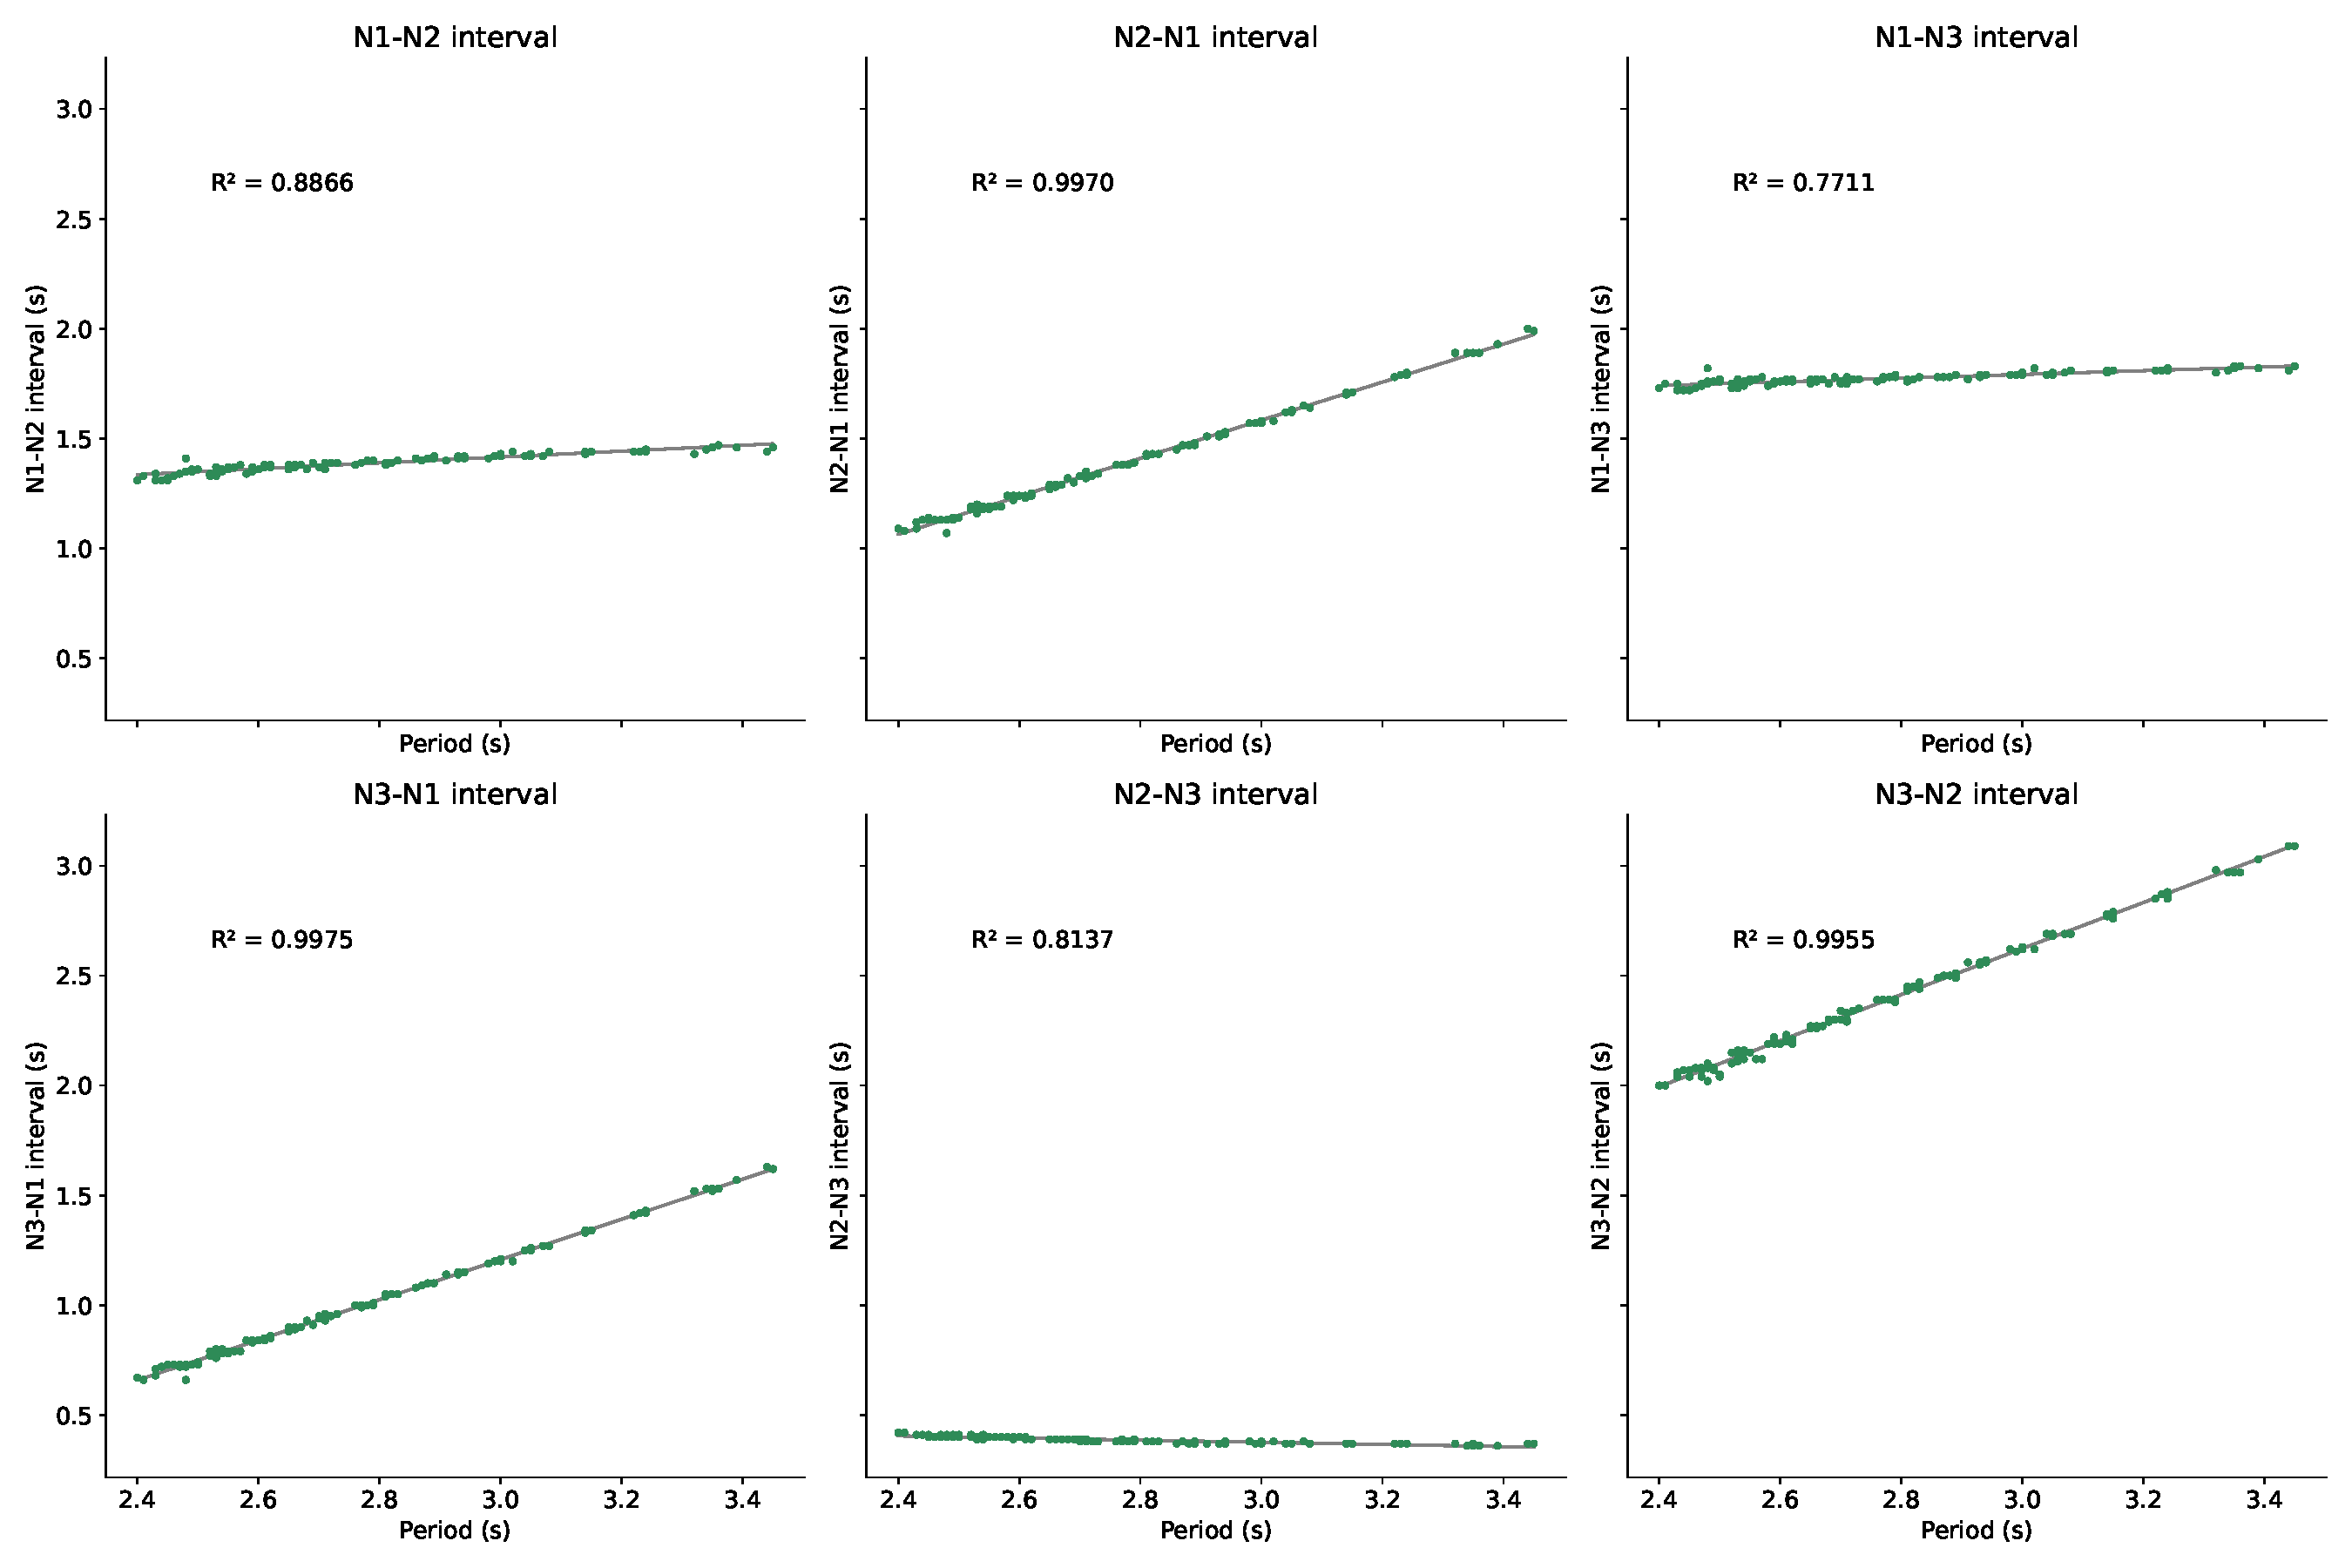
\includegraphics[width=\textwidth]{invariants/data/MODEL/n3t_driven/images/3phases/_intervals.pdf}
		\end{minipage}\
		\begin{minipage}[b]{\textwidth}
			\centering
			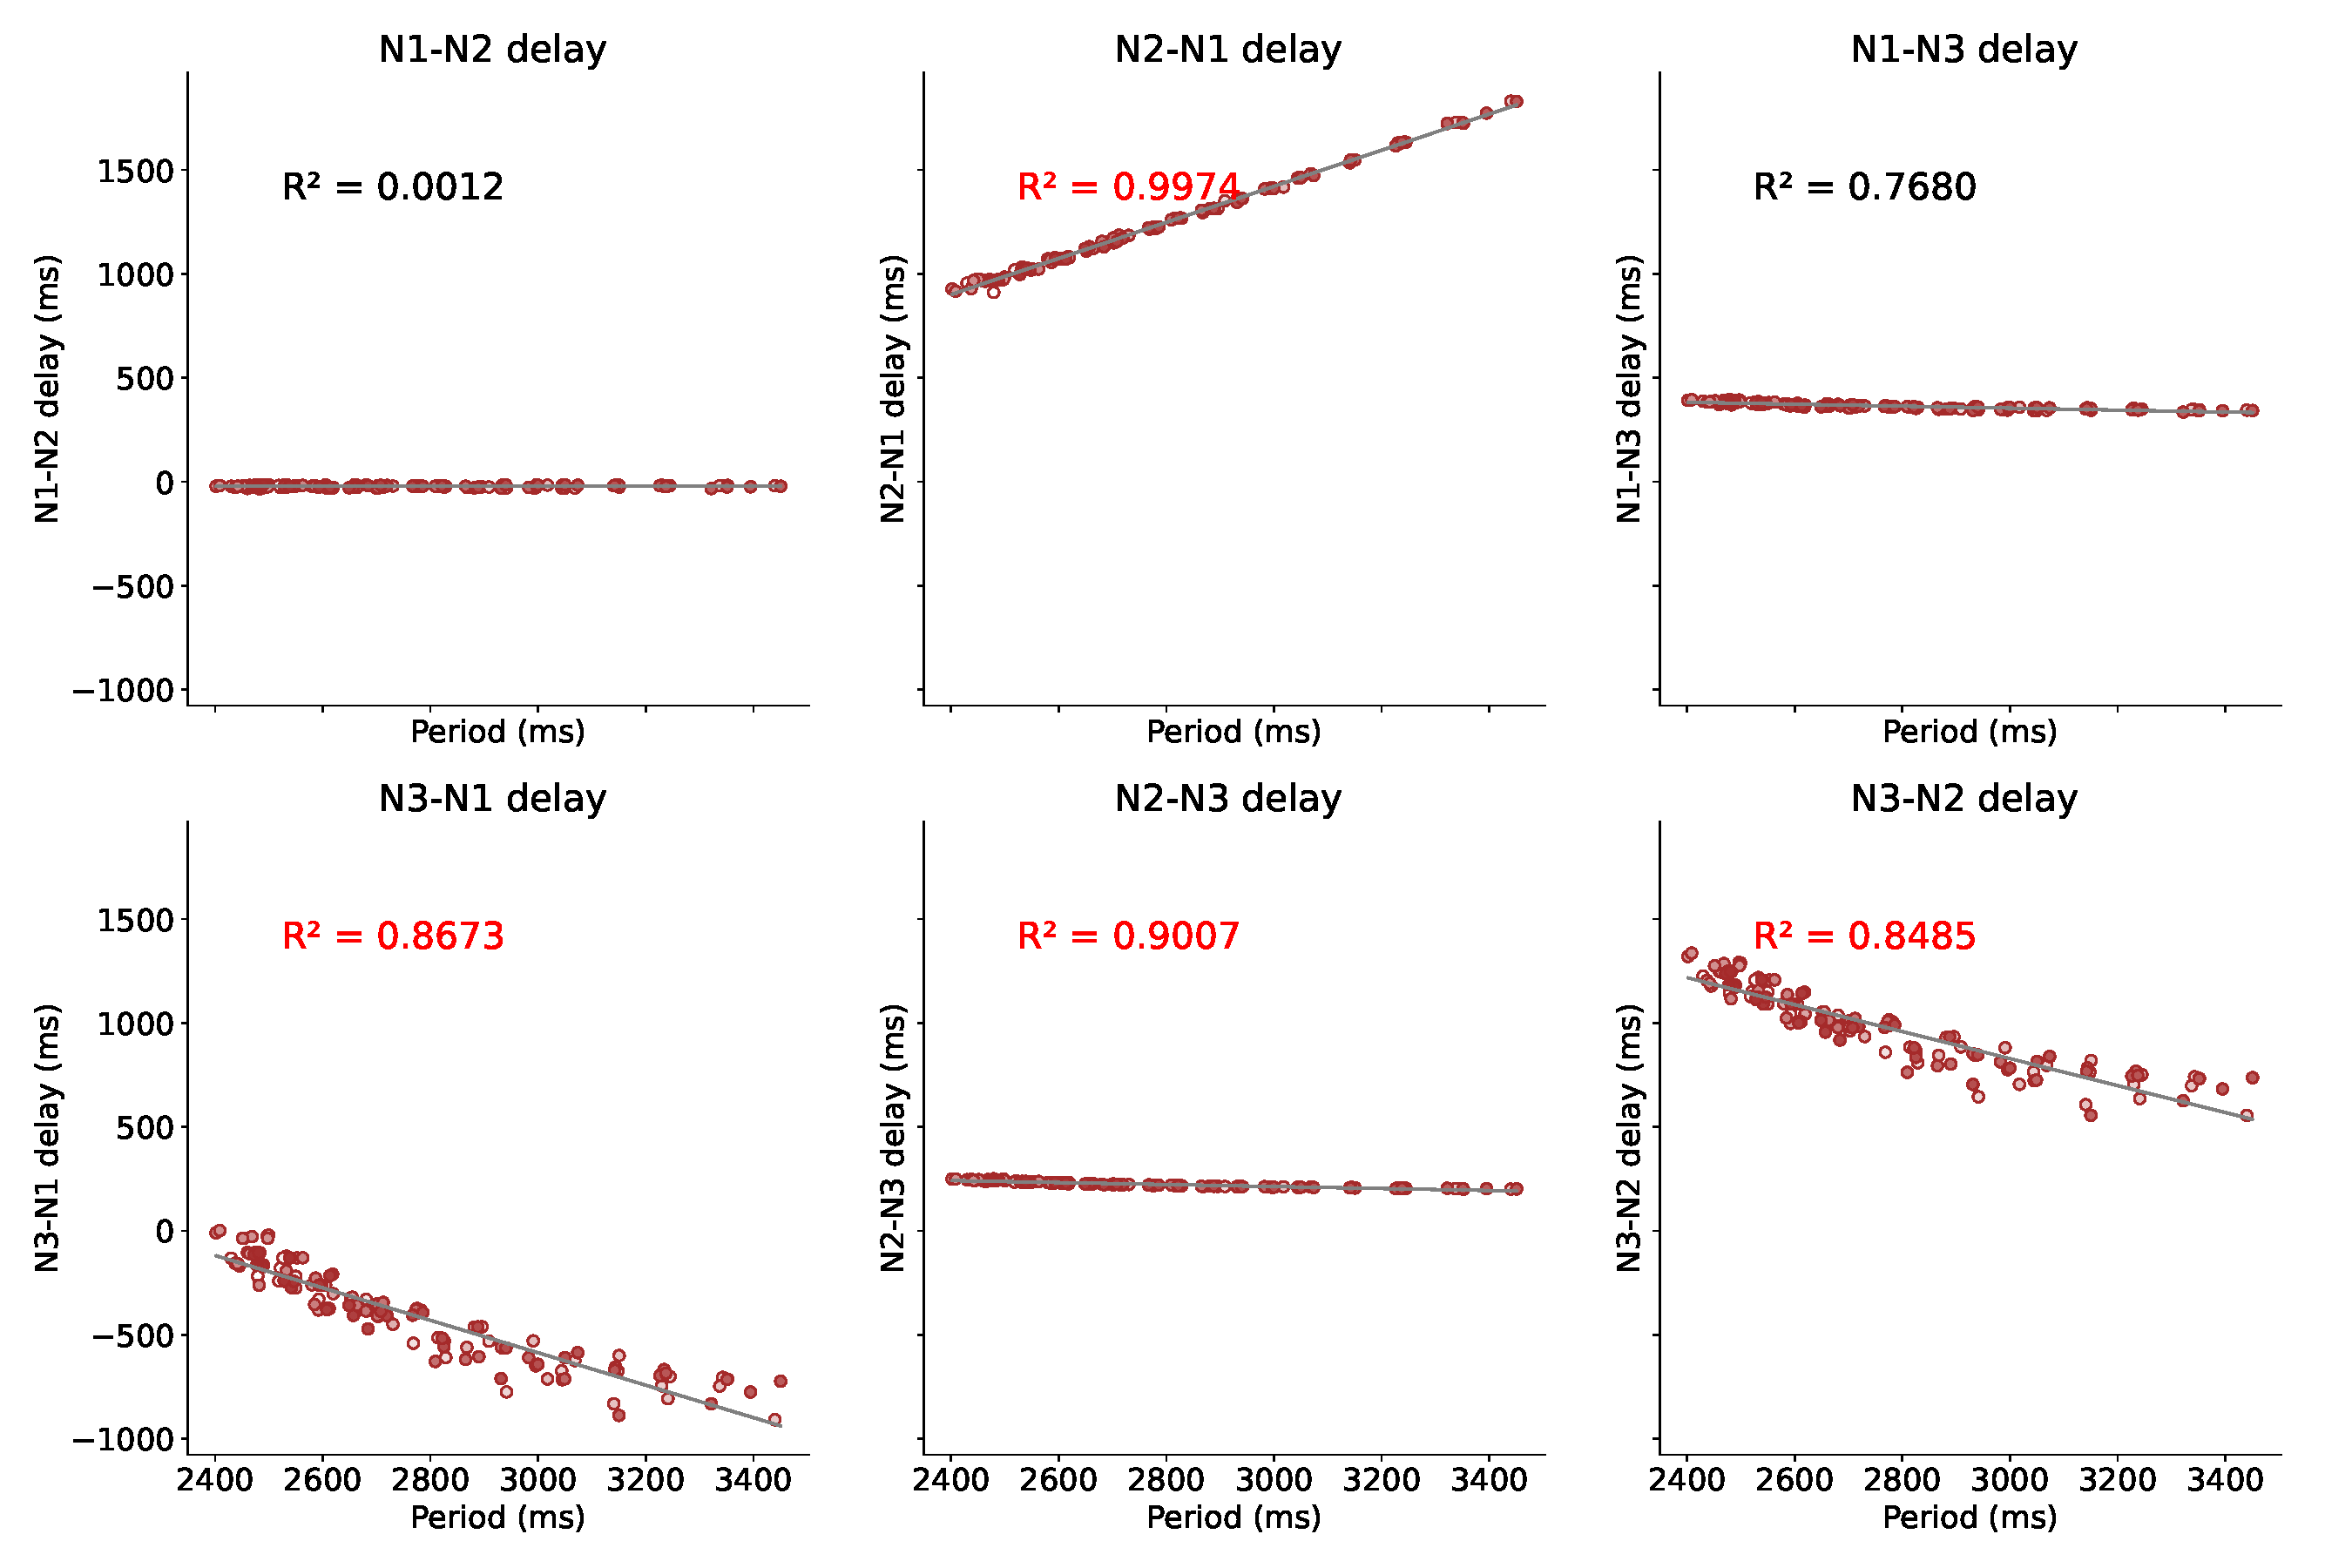
\includegraphics[width=\textwidth]{invariants/data/MODEL/n3t_driven/images/3phases/_delays.pdf}
		\end{minipage}
	\end{minipage}
	\caption{\textbf{N3t stimulation:} a) Box-plots of the sequence intervals under N3t neuron stimulation. b) Interval correlations to Period for N3t-driven simulation. First row: Burst duration. Second and third row: Two-neuron intervals. Forth and fifth row: Two-neuron delays.}
	\label{fig:invariants n3t}
\end{figure}





\subsection{SO driven variability}
\label{subsec:so driven}

The same protocol was implemented with a ramp stimulation applied to SO to induce variability, using the injected current values shown in Table \ref{table:inj values} for each neuron. Events were detected and all intervals were measured (Fig. \ref{fig:intervals}) and their variability was characterized. %This neuron has also been used in previous studies with stimulation protocols both in electrophysiological experiments and in model simulations due to its important role in rhythm activation and modulation. ***se podría quitar, si no hay que poner las referencias otra vez****

\begin{figure}[hbt!]
	\begin{minipage}[b]{0.45\textwidth}
		\centering
		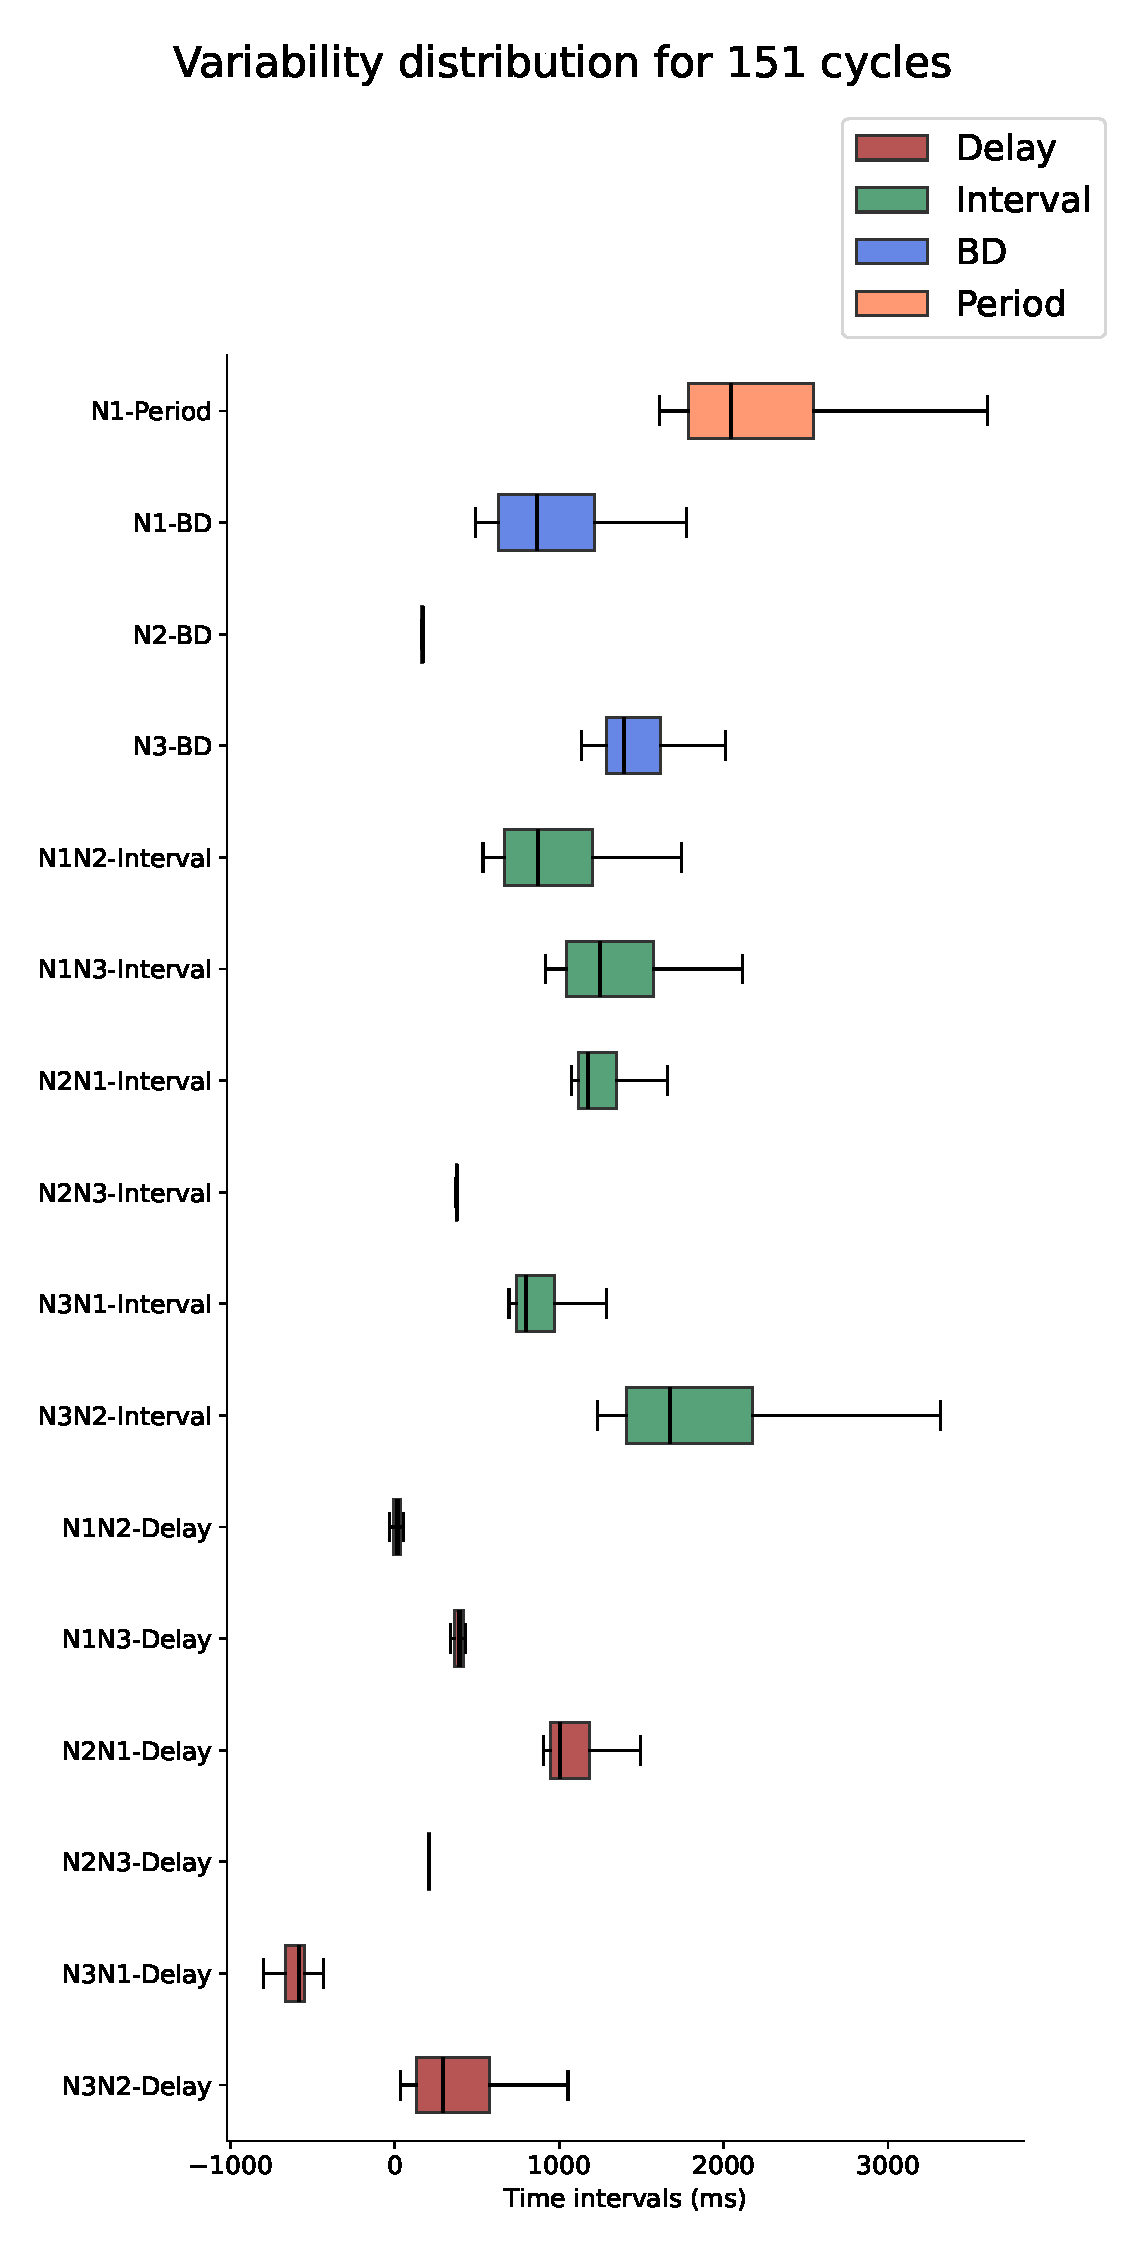
\includegraphics[width=\textwidth]{invariants/data/MODEL/so_driven/images/3phases/_boxplot.pdf}
	\end{minipage}
	\begin{minipage}[b]{0.53\textwidth}
		\centering
		\begin{minipage}[b]{\textwidth}
			\centering
			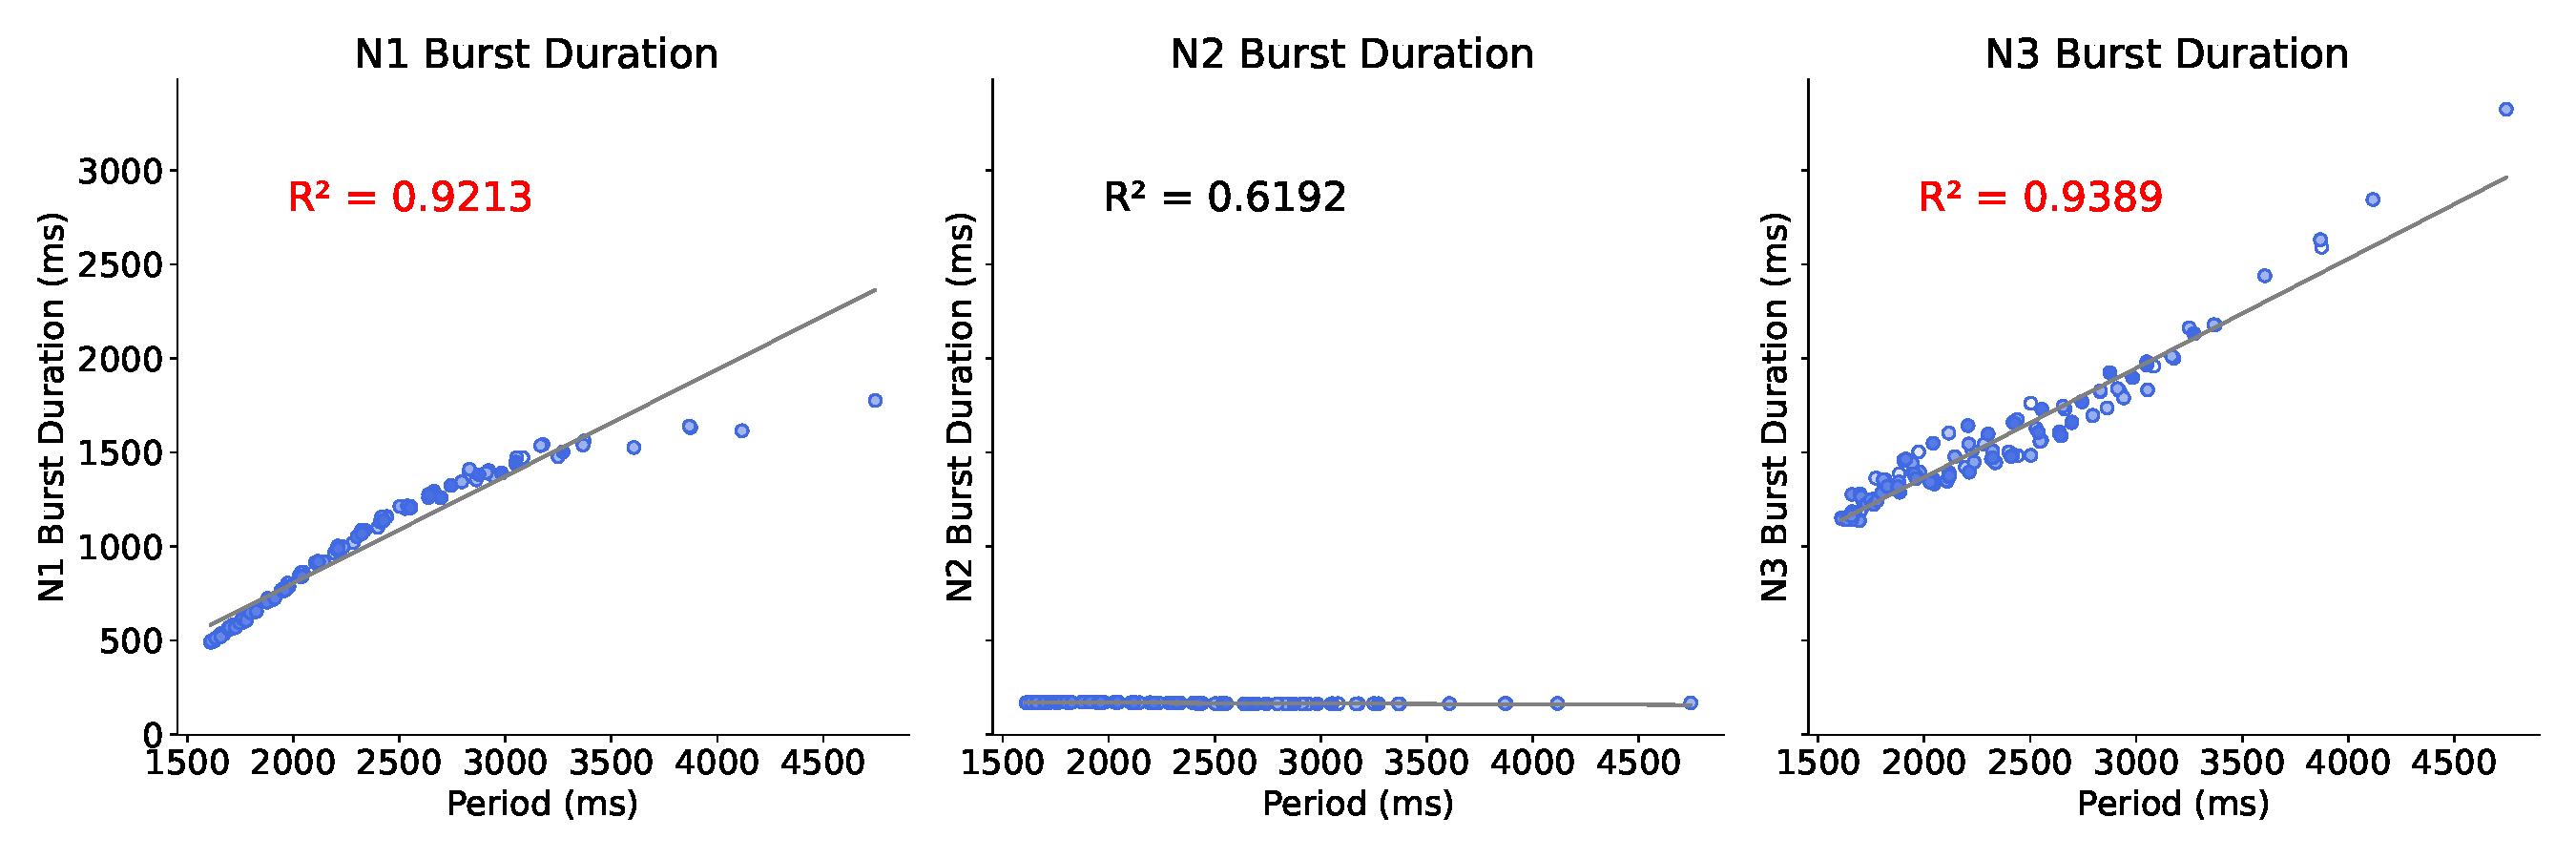
\includegraphics[width=\textwidth]{invariants/data/MODEL/so_driven/images/3phases/_durations.pdf}
		\end{minipage}\
		\begin{minipage}[b]{\textwidth}
			\centering
			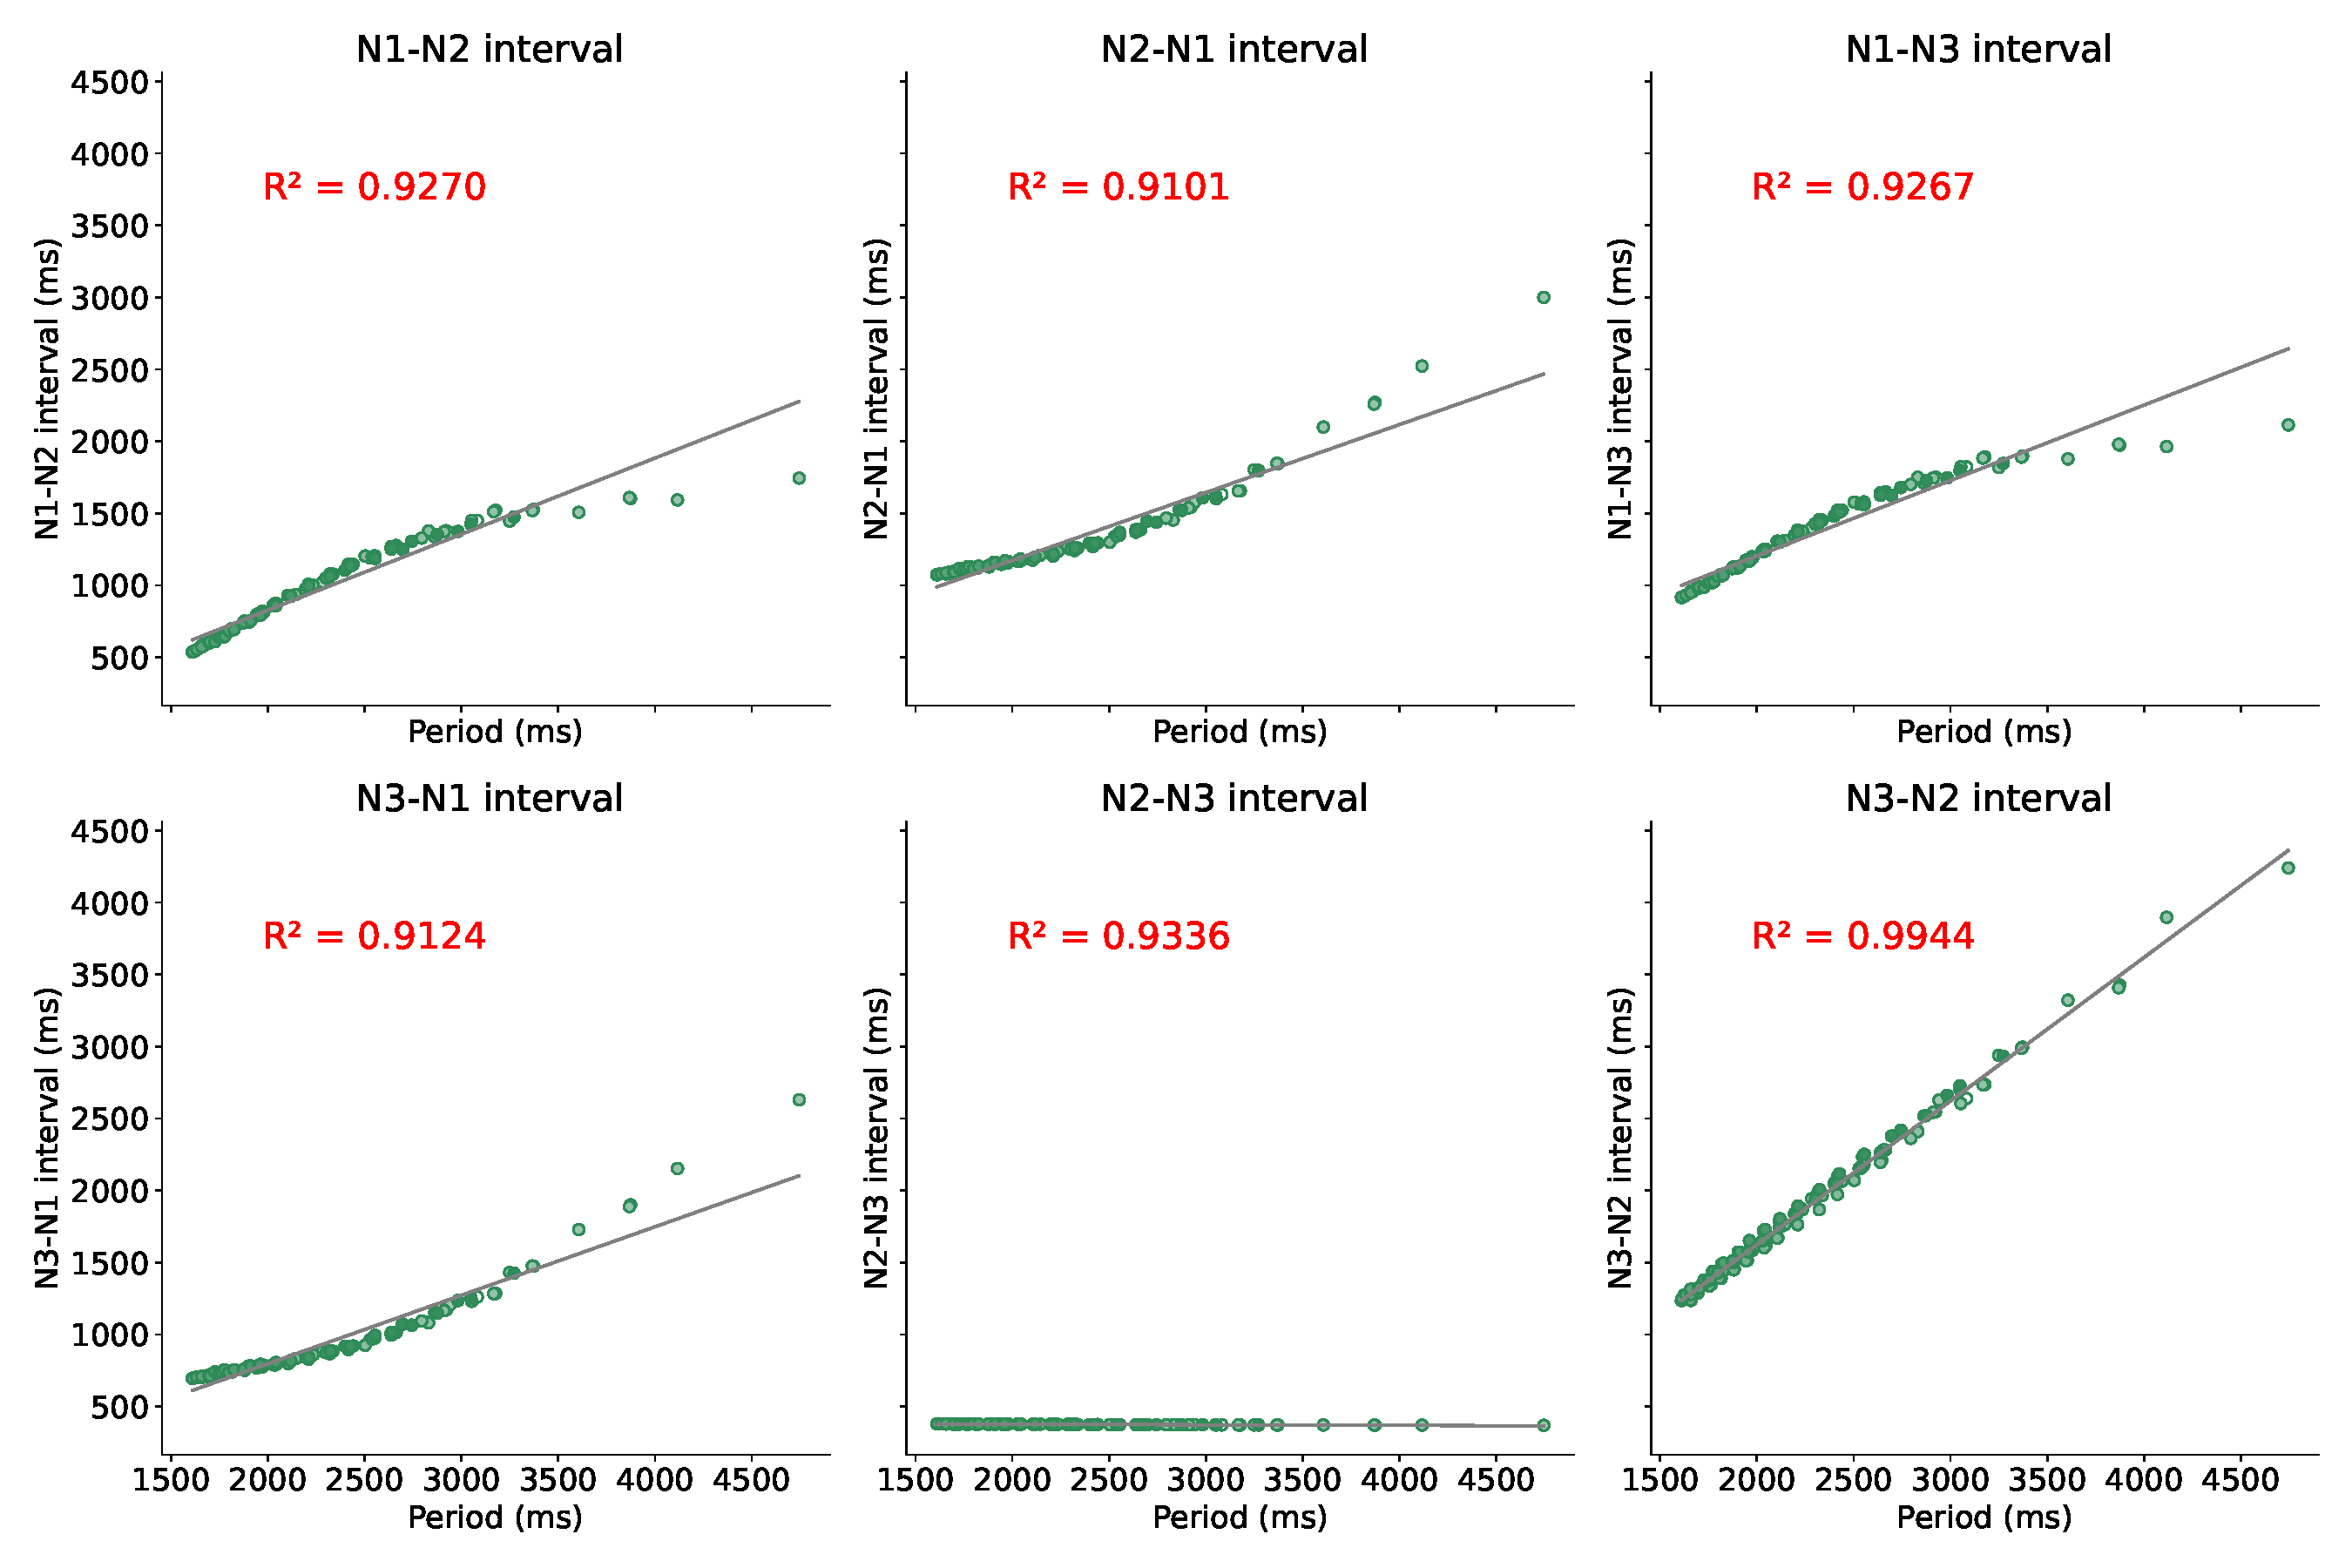
\includegraphics[width=\textwidth]{invariants/data/MODEL/so_driven/images/3phases/_intervals.pdf}
		\end{minipage}\
		\begin{minipage}[b]{\textwidth}
			\centering
			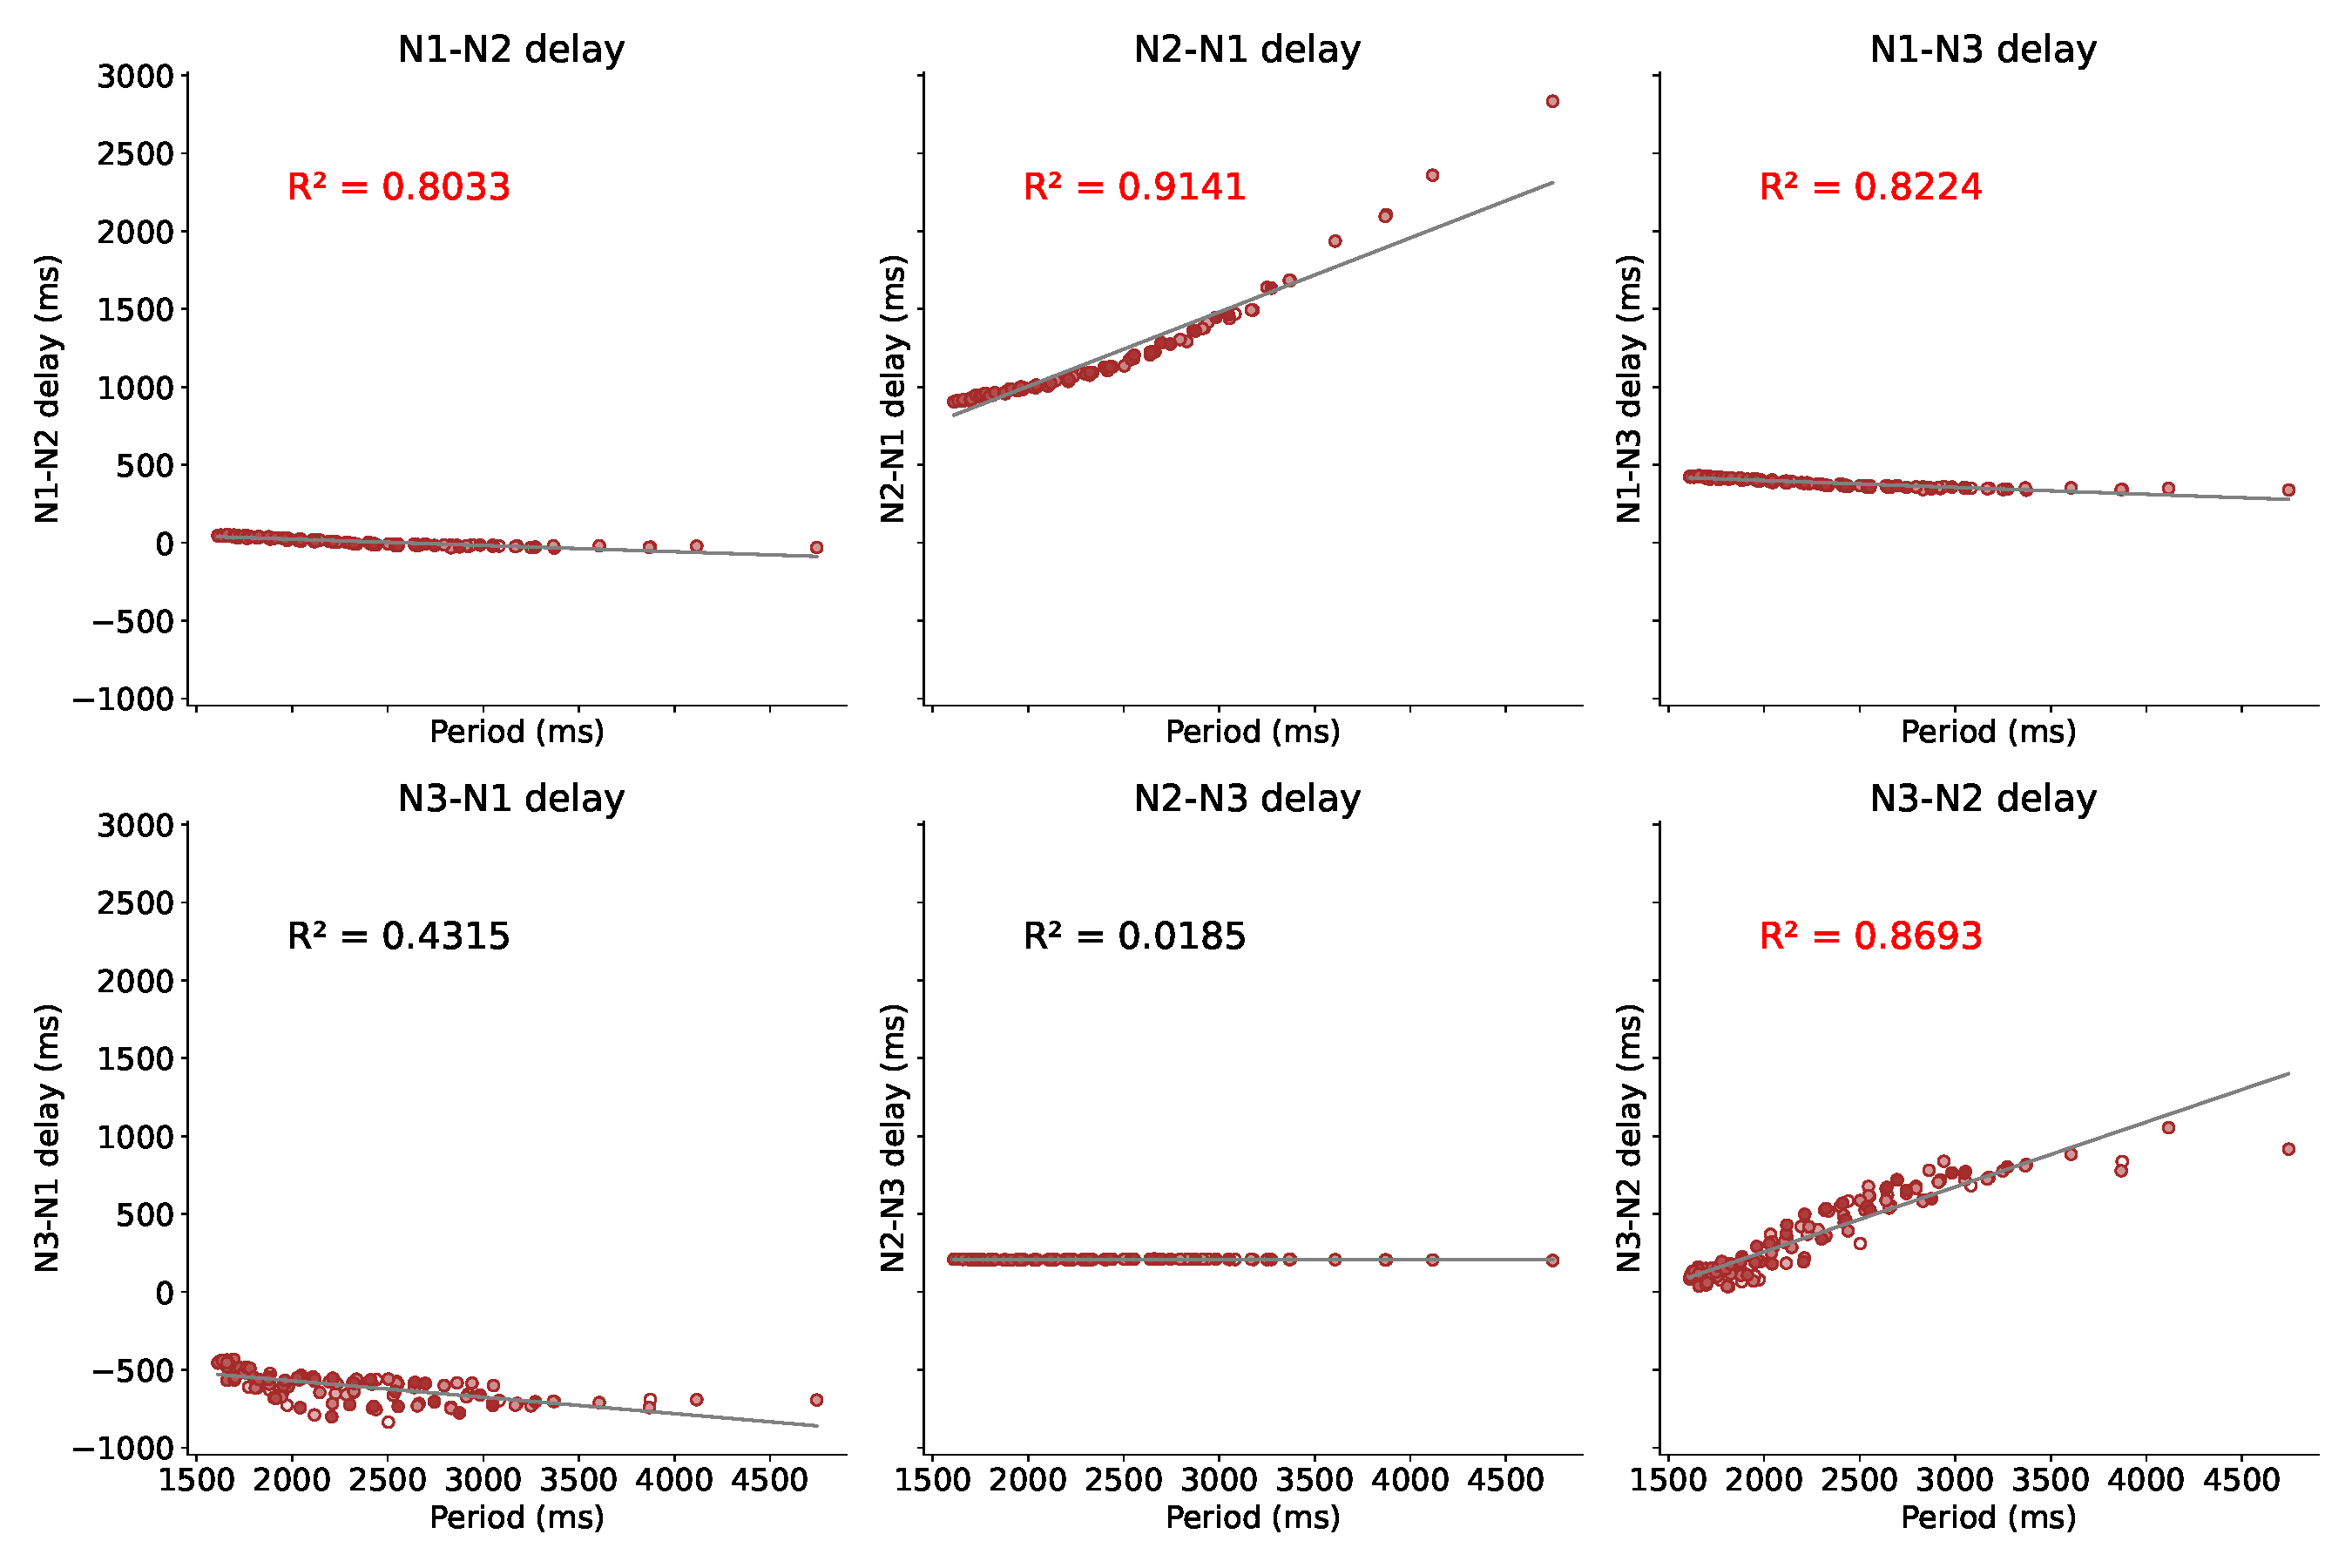
\includegraphics[width=\textwidth]{invariants/data/MODEL/so_driven/images/3phases/_delays.pdf}
		\end{minipage}
	\end{minipage}
	\caption{\textbf{SO stimulation: }a) Box-plots of the sequence intervals under SO neuron stimulation. b) Interval correlations to Period for SO-driven simulation. First row: Burst duration. Second and third row: Two-neuron intervals. Forth and fifth row: Two-neuron delays.}
	\label{fig:invariant so}
\end{figure}


Figure \ref{fig:invariant so}.a) displays the box-plot representing the distinct interval variability. In this case, we found more intervals showing large variability than in the previous cases. N2v intervals, as it happened in the previous results, show low variability. %, which indicates that period variability is more likely a consequence of N3t and N1M activity.
N1M and N3t neurons show high variability in their burst duration intervals, being N1M even more variable than N3t, as opposed to the previous results when the stimulation was introduced in other cells. All intervals derived from these two neurons have high variability and a similar structure. %Therefore, now the intervals which show low variability are the ones related to N2v. 

% In spite all this, what remains constant from N1M-driven simulation is the variability of the N3-N2 interval, which includes both N1M and N3t burst duration, being N3-N2 the most variable one, and the closest to the period variability.%distribution

% Since in this case there are more neurons showing high variability, we should expect finding more correlations when plotting each interval against the period.  ***también deberíamos quitar redundancia aquí***
% Hence, as it happened in the previous results, all intervals related to N3t show dynamical invariants, but this time they are also present in the ones related with N1M, which show a high variability. 
% the intervals with more variability and, thus, those that had a more similar variability structure to the period, were the ones that showed dynamical invariants%(a highest linear relation to the period)


Figure \ref{fig:invariant so}.b) displays the corresponding correlation analysis between all intervals and the period. %In this case, as it happens in the box-plot, there are found different results
In this case, we found correlations in the same intervals as before: N2-N1, N3-N1, N3-N2 intervals and N2-N1 delay; which are the intervals related to N3t burst duration. However, under SO stimulation,  N1-N2, N1-N3 intervals were also highly correlated to the period. Even the correlation for N3-N2 delay considerably increased in relation to the other stimulation conditions. These intervals are the ones related to N1M neuron activity, and were also the most variable ones.  These results reproduce the experimentally analyzed effects set out in \parencite{elliott_temporal_1991}, when rhythm and variability was induced by injecting current into a living SO neuron.

%Furthermore, it is important to notice that N3-N1 delay is negative again ****por qué es importante si es lo mismo que antes****. As it happened in N3t-driven simulation, this means there is a constant overlapping between N3 and N1 in each cycle, i.e. N3t burst interval is coming earlier. This can be also appreciated in boxplot, since this interval is represented below 0. 

Compared to the N1M and N3t stimulation results, there is another difference when driving the rhythm with SO: burst duration is much shorter, so the period and the rest of intervals are consequently smaller. Therefore, when driving the rhythm by SO, the period variability seems to arise from both N3t as well as by N1M. 
%the model produces a rhythm where the information about period duration seems to be carried by N3t as well as by N1M. 



\subsection{Cycle-by-cycle time intervals relations not only involving the period}
We have discussed so far the sequential dynamical invariants in terms of strong linear relationships between the distinct intervals in a cycle and the period.  However, studying the relations between all possible combinations between intervals can also show interesting information about the temporal variability distribution in the ongoing sequential activity. Figures \ref{fig:model n1m stimulation pairplot} to \ref{fig:model so stimulation pairplot} provide a representation of all these combinations of the defined intervals for the three scenarios of induced variability (current in N1M, N3t or SO) discussed in this section. In this extended representation of the cycle-by-cycle relationships, we can see that there are multiple intervals presenting strong linear relations in addition to the periods. Some of them are intervals that are contained within others, as in the case of N1-BD and N1-N2 intervals, which have similar durations, and so they are more likely to have a strong linear relation between them. However, there are other intervals that, although they share part of the time-interval, they are not correlated. This was the case of the N2 burst duration with the period, that burst duration was contained in the period but it had no relation to it. And we also observe this in the relation of N2-BD with N2-N1 interval. This distinction can help dissecting the source of variability and its distribution when an interval is related to the period. Also, a further study of linear relationships between  intervals (such as N1-BD and N3-BD) that do not share any other common time-interval, can show significant information about the ongoing cycle-by-cycle activity. This representation can also show non-linear relations between the intervals, as we can see in some plots in the case of SO (Fig. \ref{fig:model so stimulation pairplot}). These nonlinear relationships have been observed in the pyloric CPG both in modeling and experimental scenarios \parencite{berbel_emergence_2024}.

\begin{figure}[htbp]
	\centering
	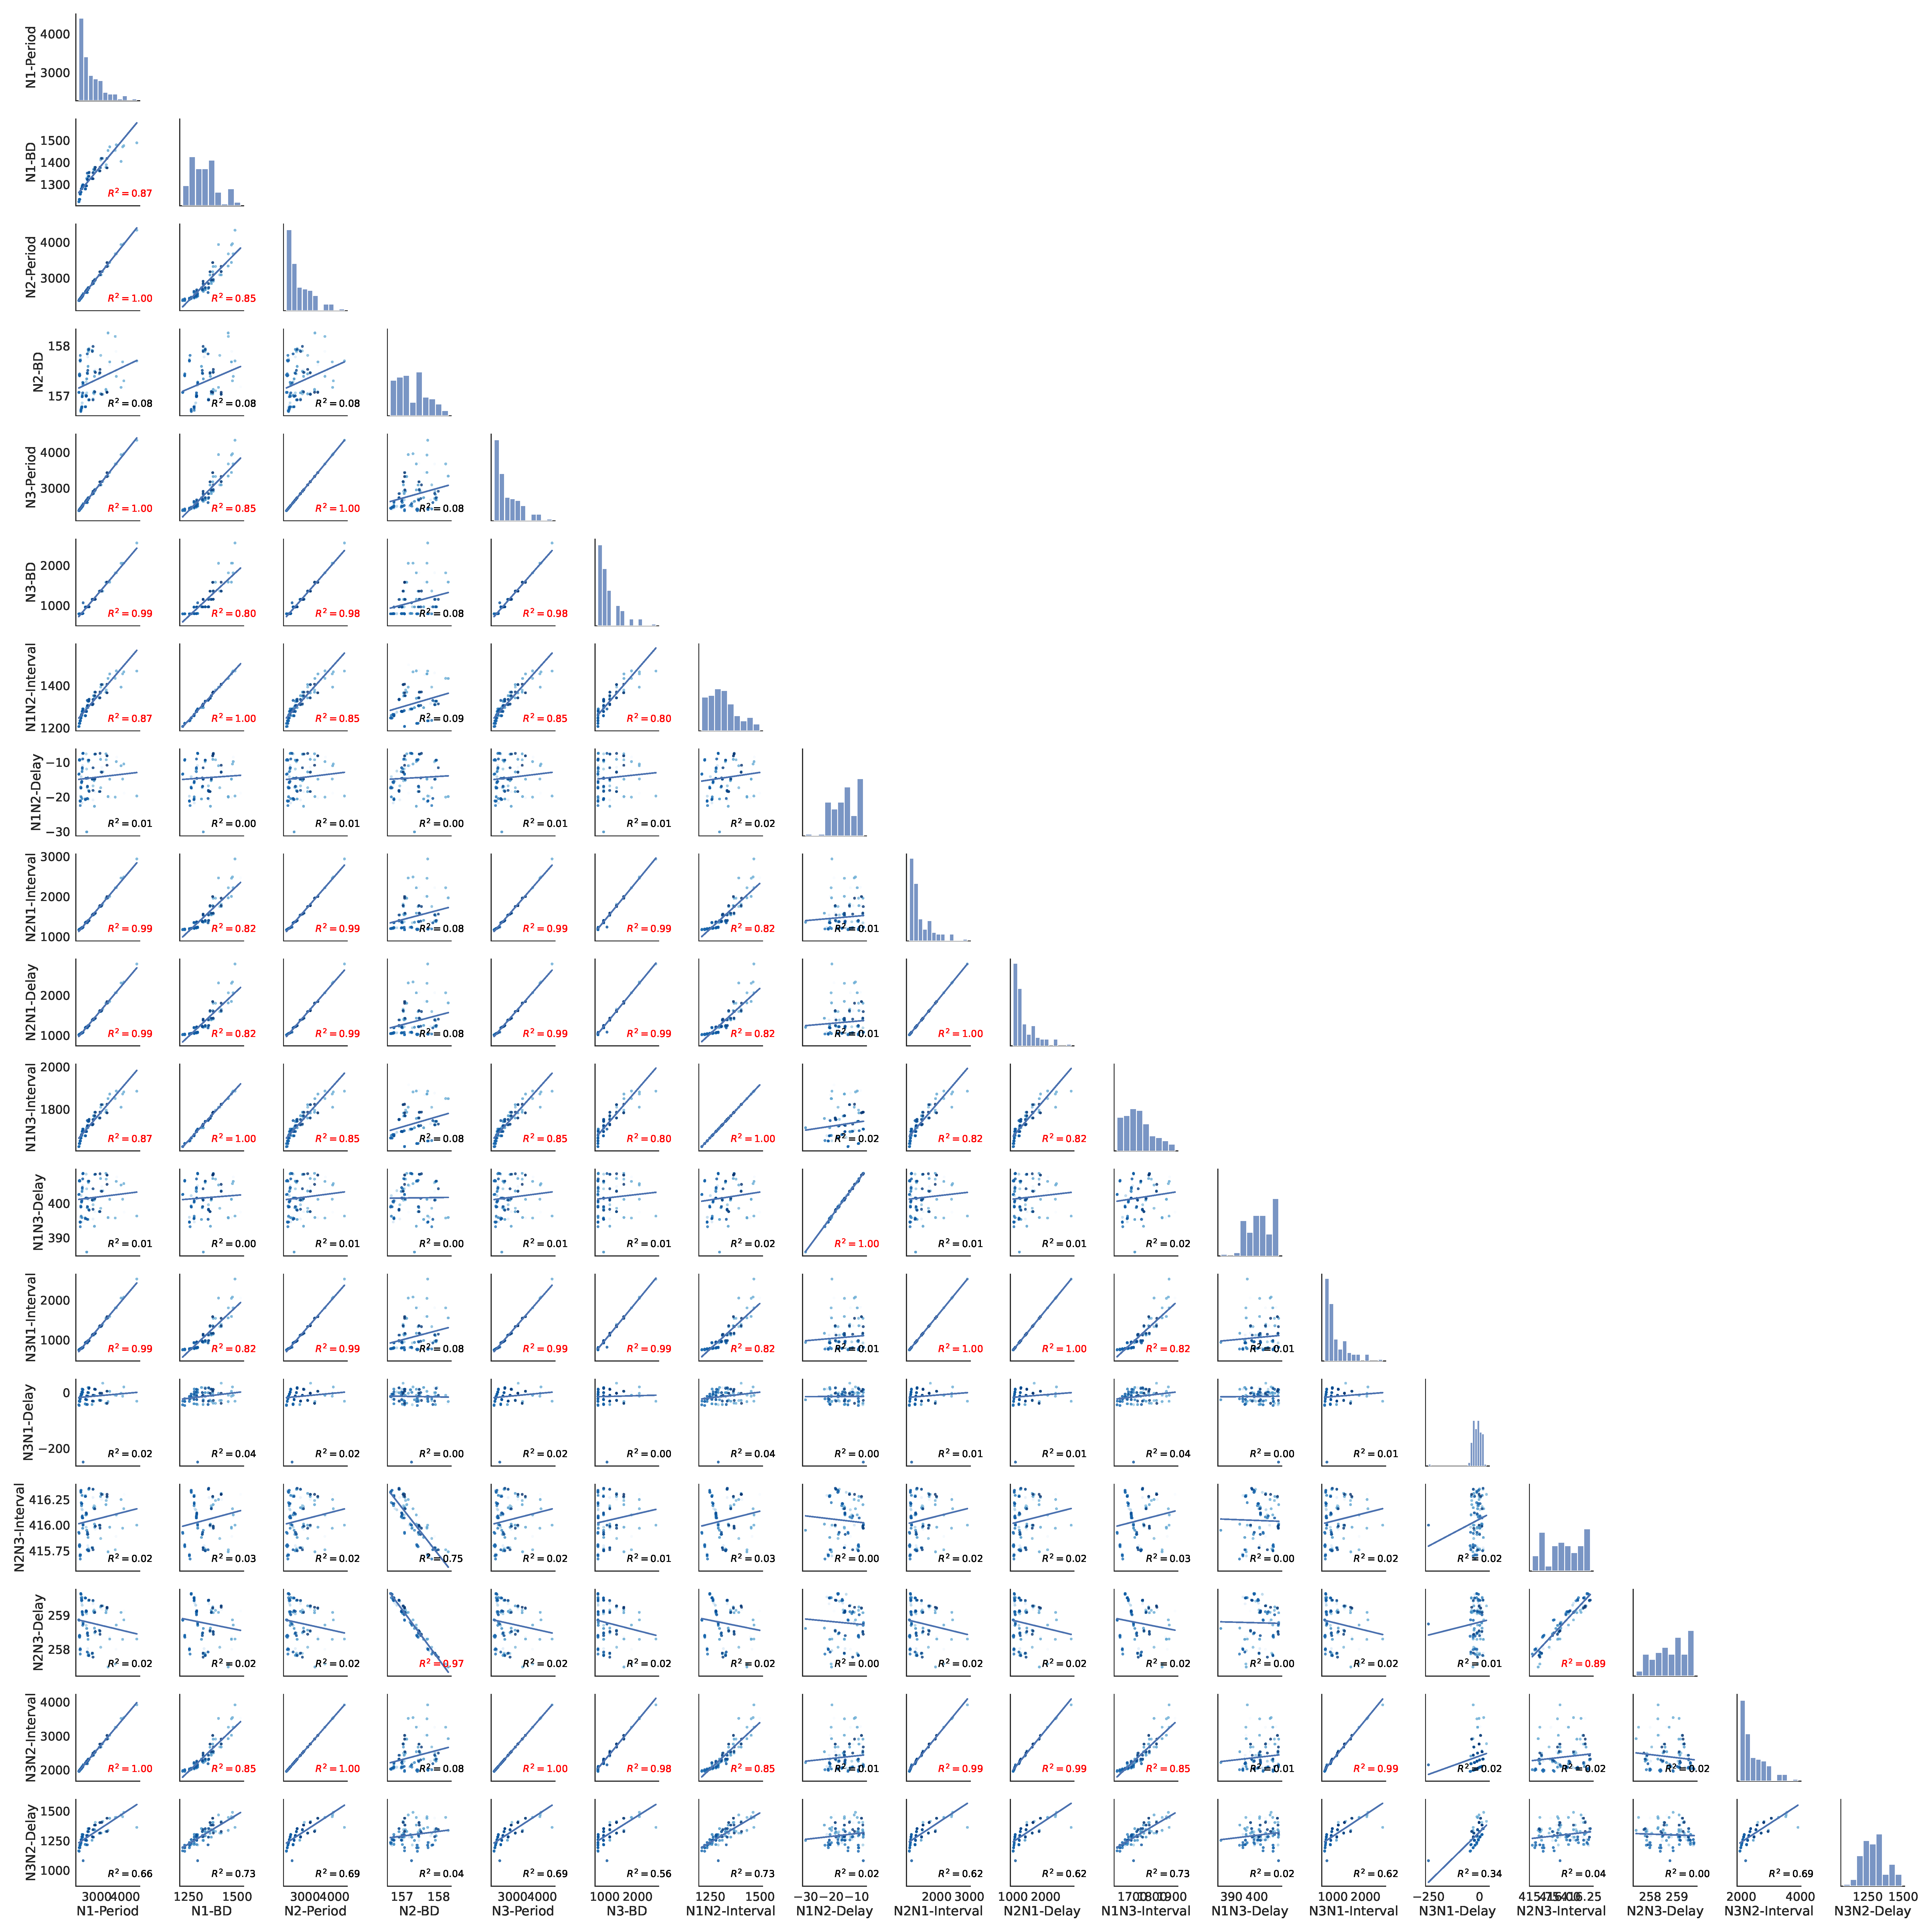
\includegraphics[width=\textwidth]{./invariants/data/MODEL/n1m_driven/images/3phases/output_pairplot.png}
	\caption{\textbf{N1M stimulation}: Pairplot with all possible combination between time intervals within a cycle.}
	\label{fig:model n1m stimulation pairplot}
\end{figure}
 
\begin{figure}[htbp]
	\centering
	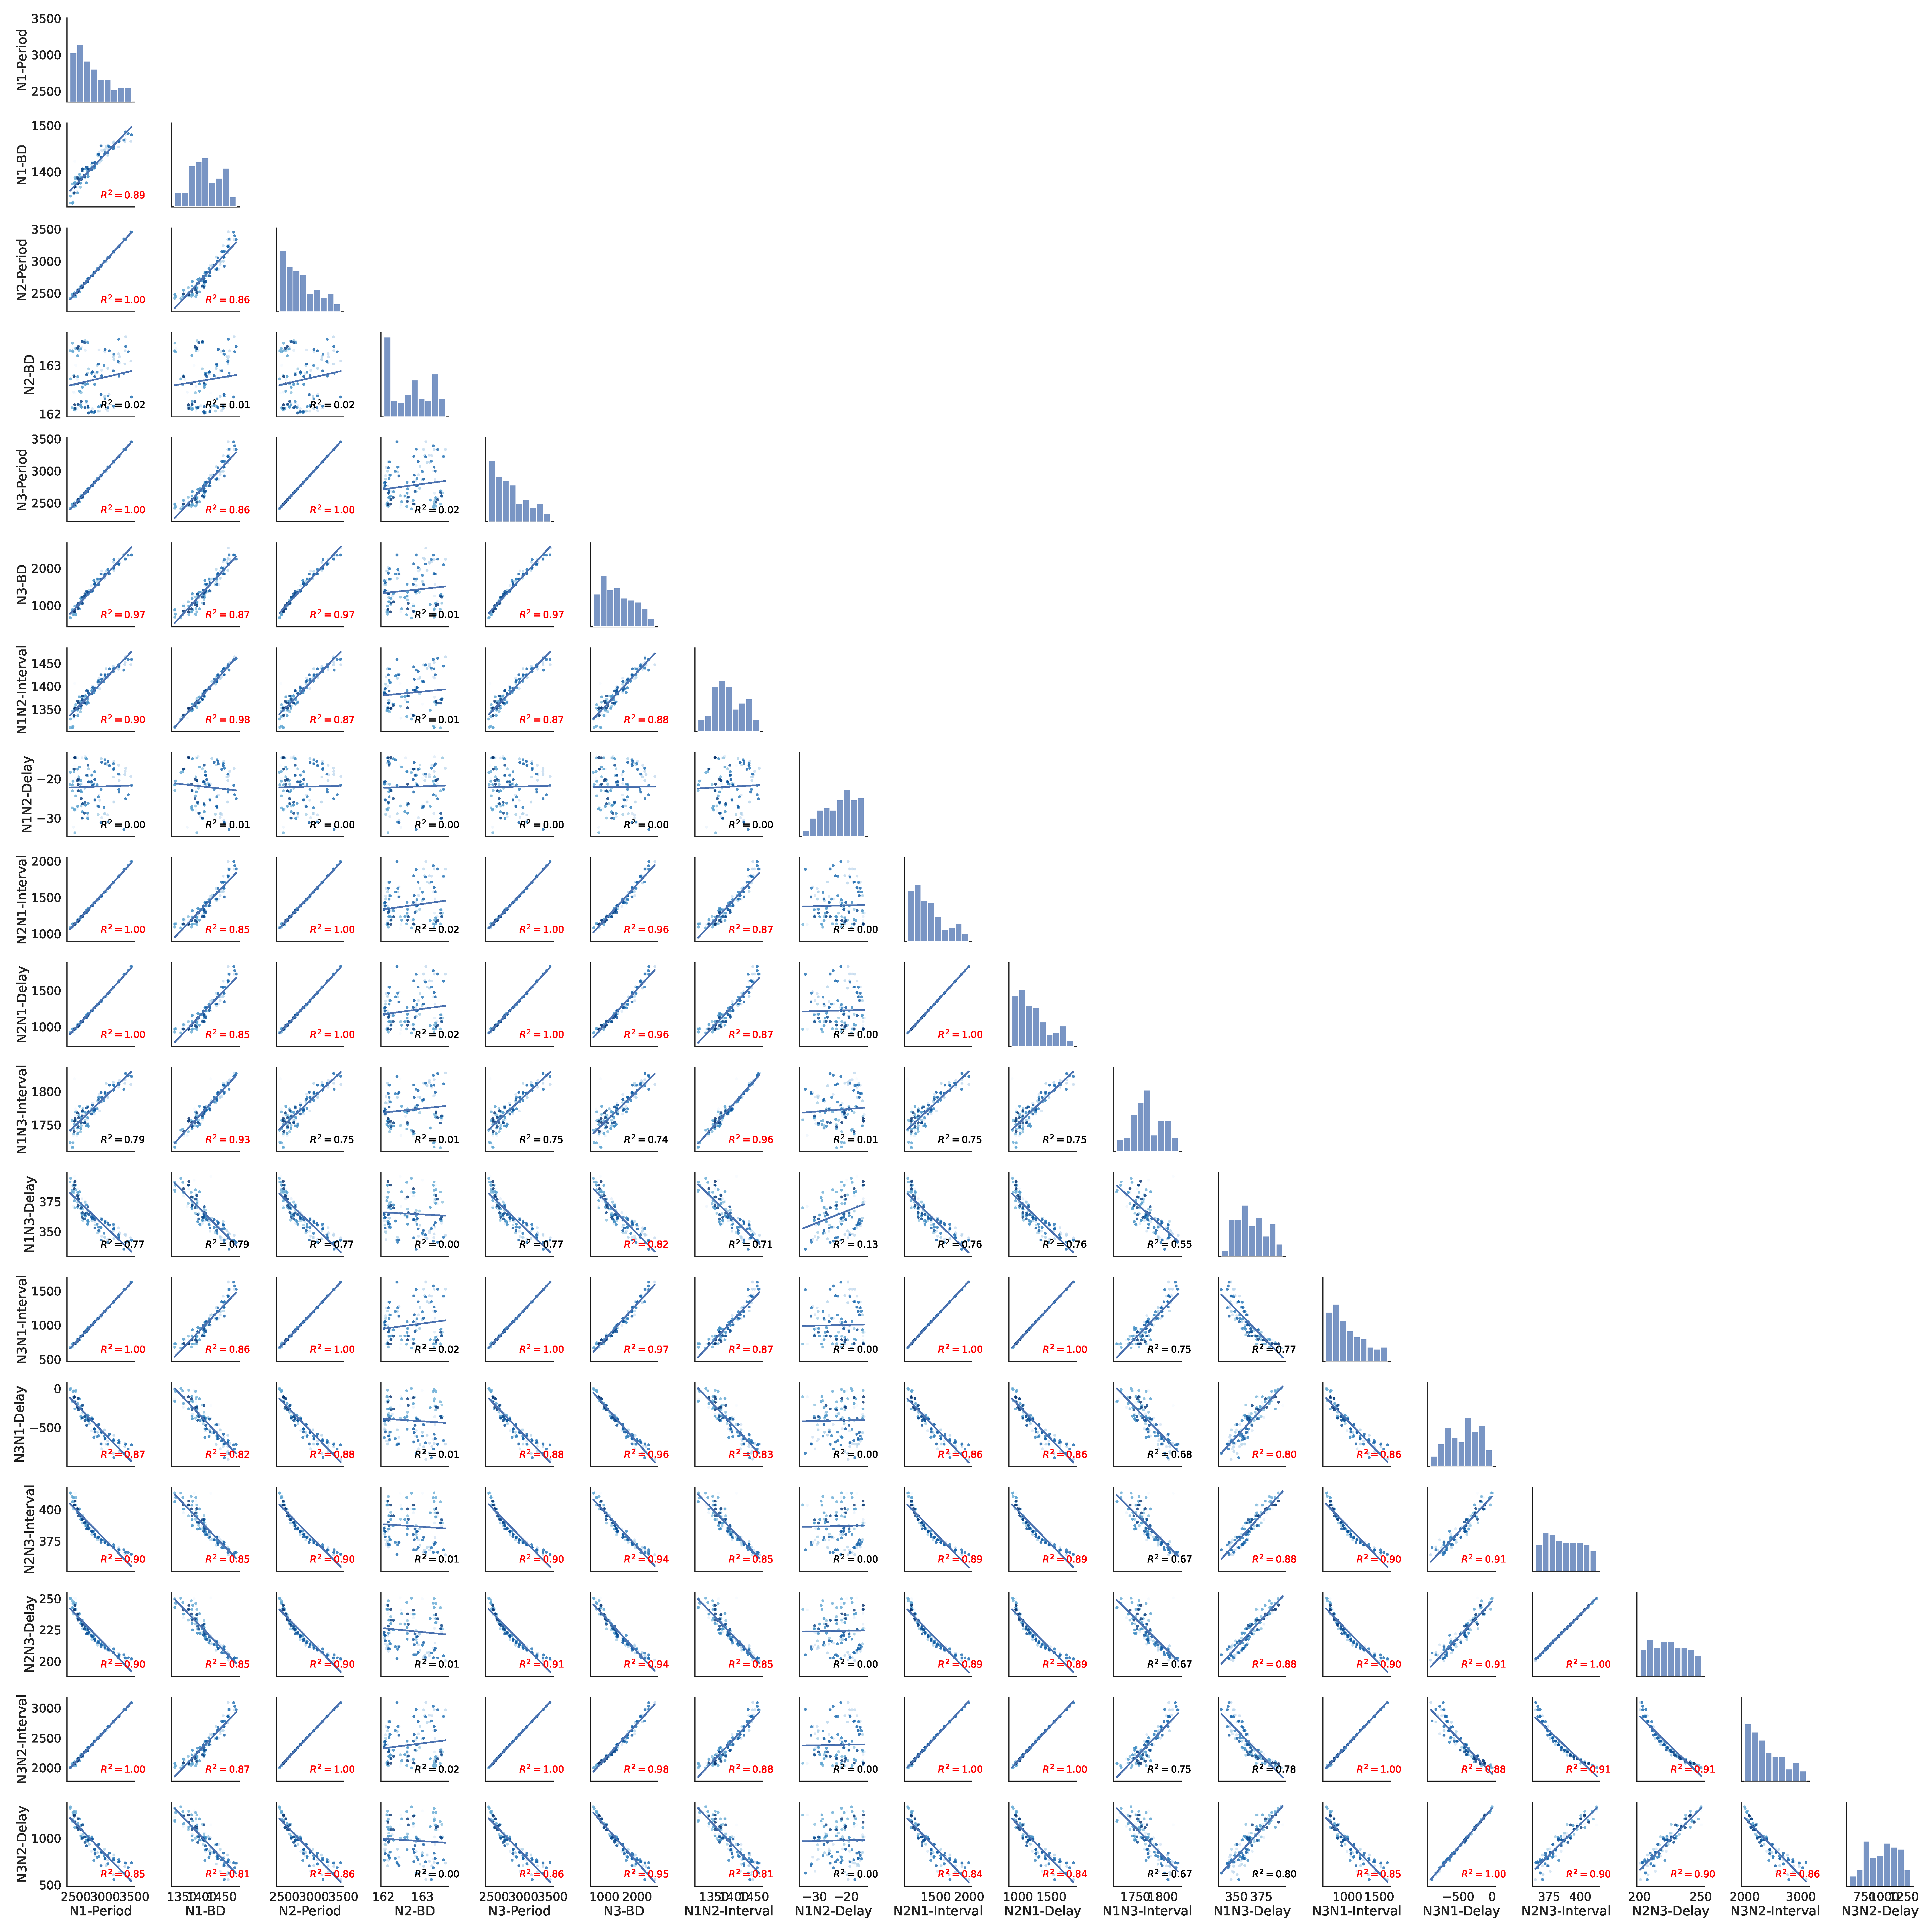
\includegraphics[width=\textwidth]{./invariants/data/MODEL/n3t_driven/images/3phases/output_pairplot.png}
	\caption{\textbf{N3t stimulation}: Pairplot with all possible combination between time intervals within a cycle.}
	\label{fig:model n3t stimulation pairplot}
\end{figure}

\begin{figure}[htbp]
	\centering
	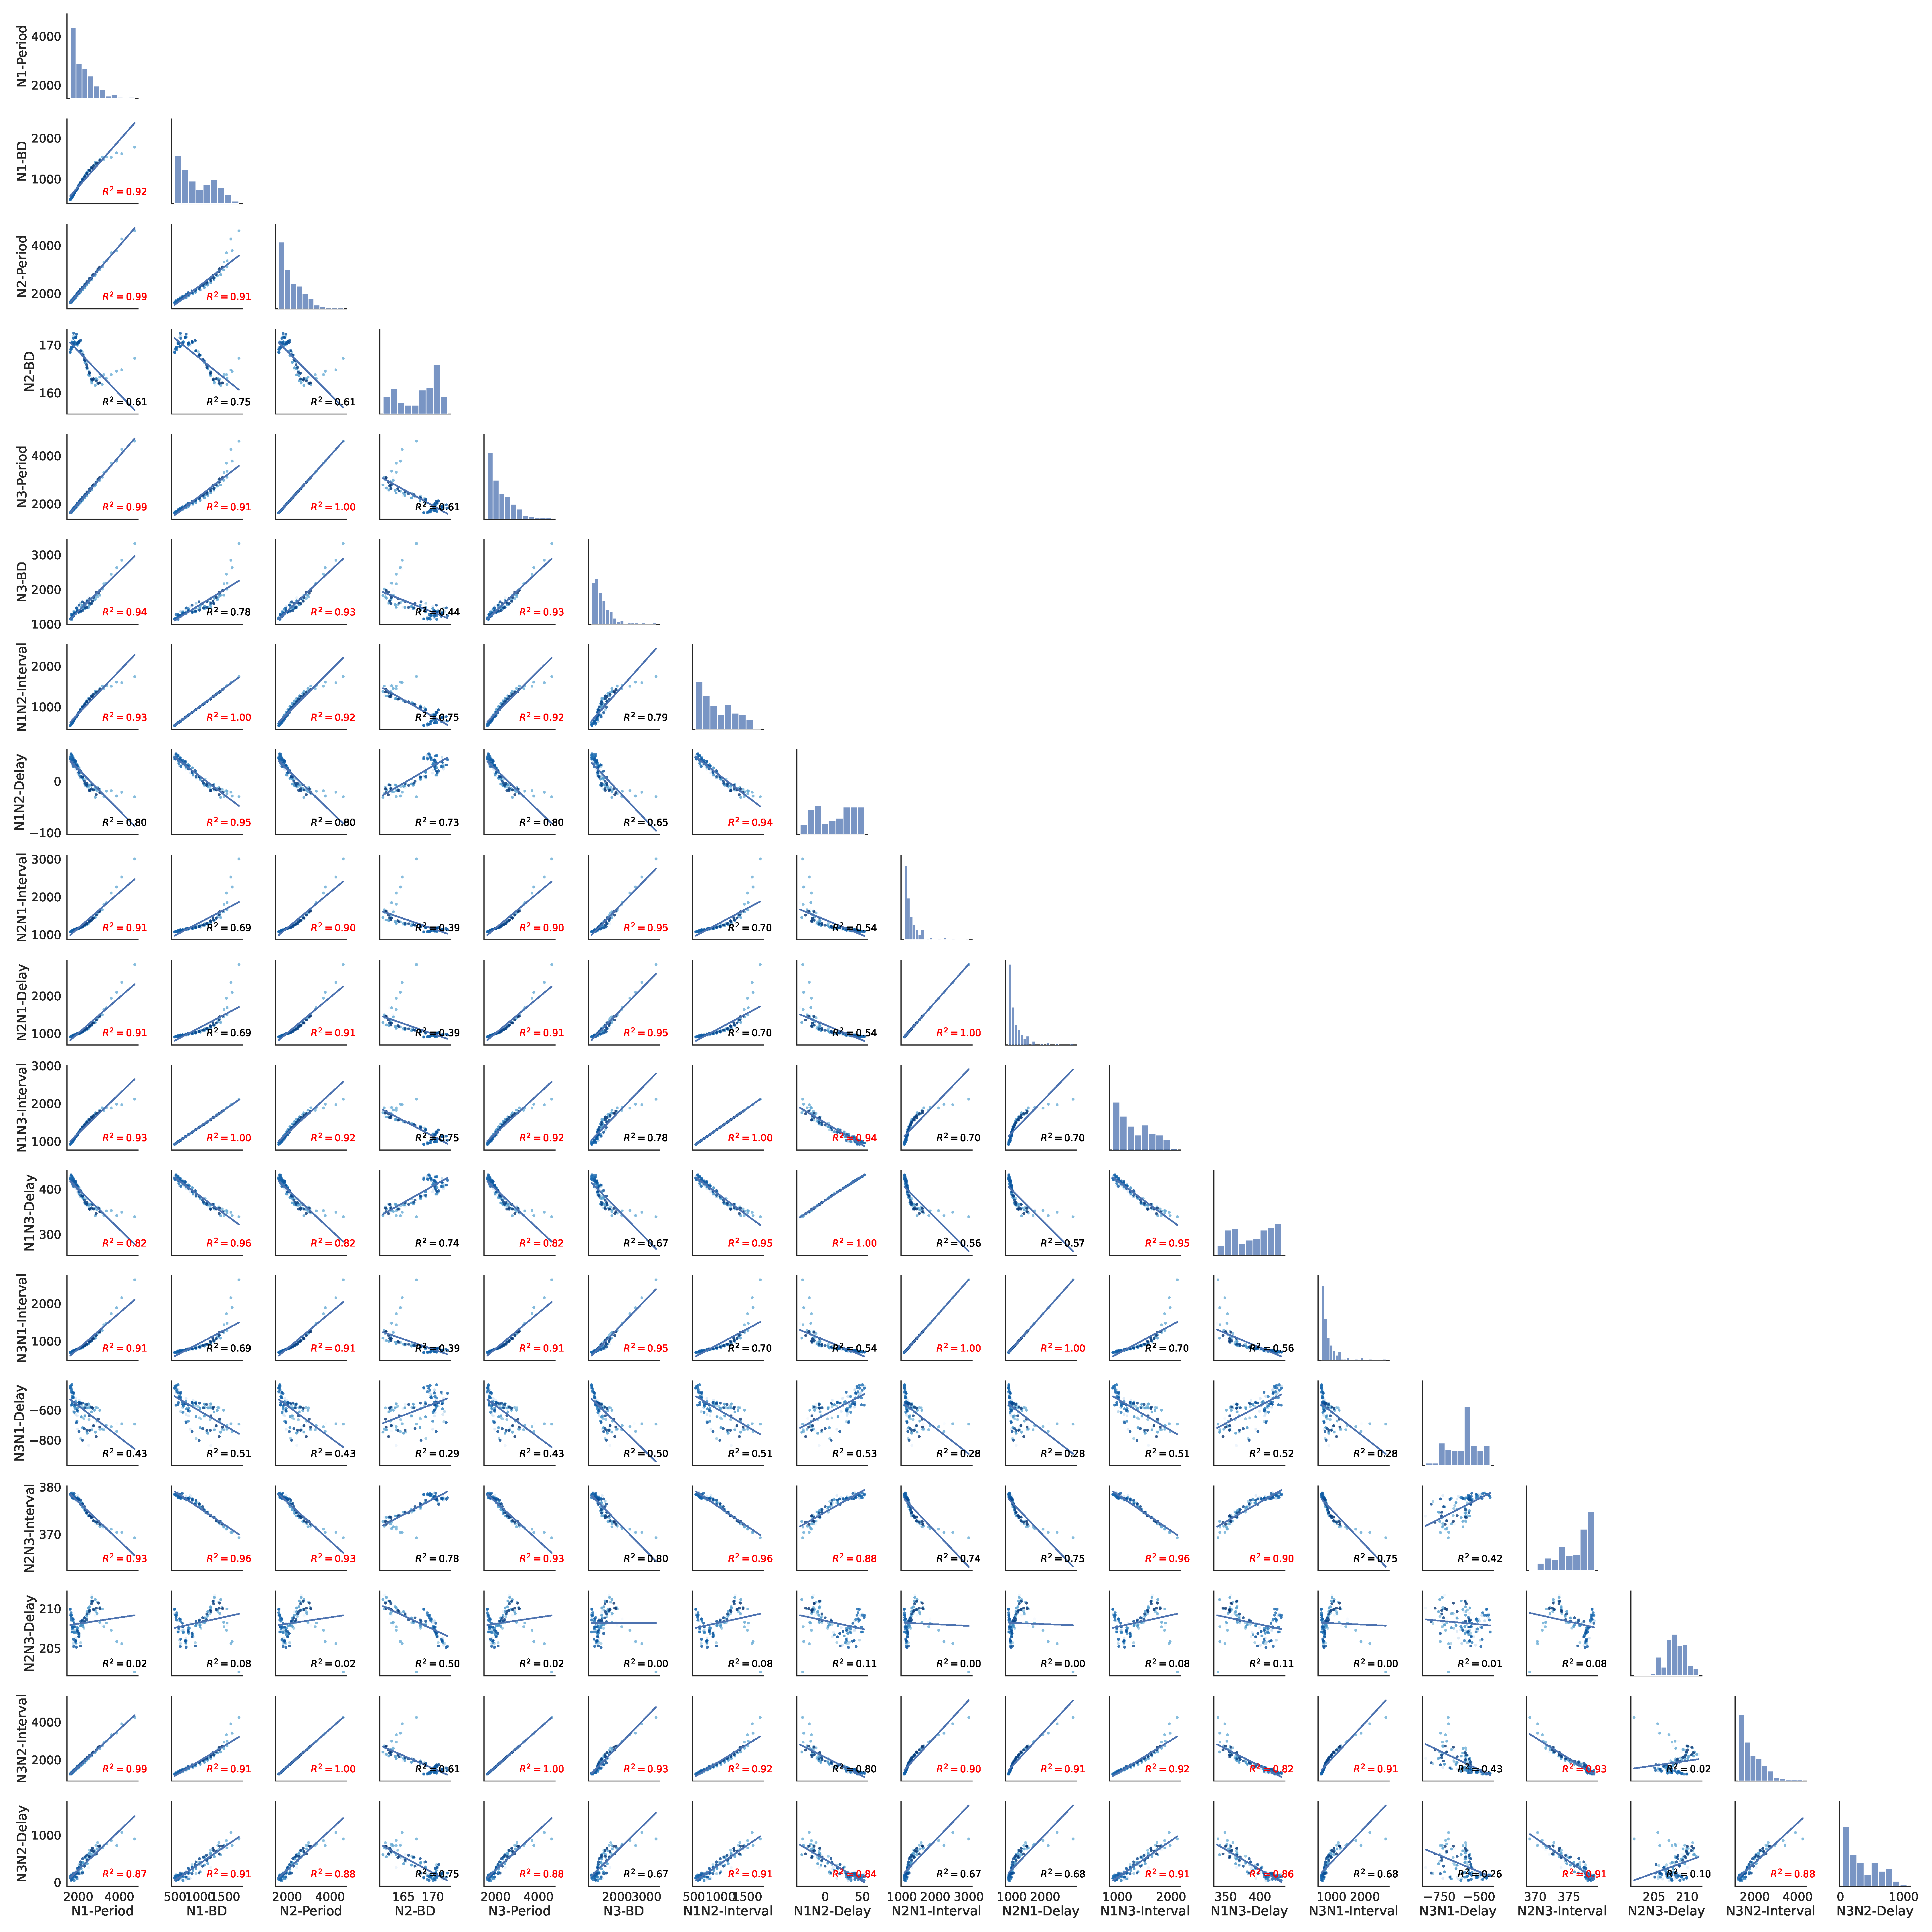
\includegraphics[width=\textwidth]{./invariants/data/MODEL/so_driven/images/3phases/output_pairplot.png}
	\caption{\textbf{SO stimulation}: Pairplot with all possible combination between time intervals within a cycle.}
	\label{fig:model so stimulation pairplot}
\end{figure}

%
\subsection{Comparison with two-phase intervals}
In the previous subsections, we analyzed the sequential dynamical invariants for three phases, but we can also define two-phase intervals, taking as reference for example, N1 and N3. This is the case discussed in the work by \textcite{elices_robust_2019}, and in the following section we will also use two phases for some of the recordings were it was not possible to characterize the N2 phase out of the intracellular recordings. Figure \ref{fig:invariant n1m model 2 phases} provides a comparison of  different intervals conforming the sequence and associated relationships when the time references are set in N1, N2 and N3 (as we have shown so far) or only for N1 and N3.

When we only consider two phases, we have less possible combinations and the time-intervals that would correspond to the third neuron are contained in the resulting ones. For example as we can see in Fig. \ref{fig:invariant n1m model 2 phases}a), N2N3 delay would be represented by N1N3 delay and N2 burst duration is included in the N2N3 interval. This result is relevant when analyzing two-phase intervals in the case triphasic rhythms.
%Thus, when analyzing dynamical invariants in two-phase intervals, each interval is more informative of the variability constrains cycle-by-cycle. 

\begin{figure}[hbt!]
	\begin{minipage}[b]{0.9\textwidth}
		\raggedleft
		\begin{minipage}[b]{0.53\textwidth}
			\raggedleft
			\begin{overpic}[width=\textwidth]{methods-paper-modelo/Intervals_figure_complete.png}
				\put(0,40){\large\textbf{a)}}
			\end{overpic}
%			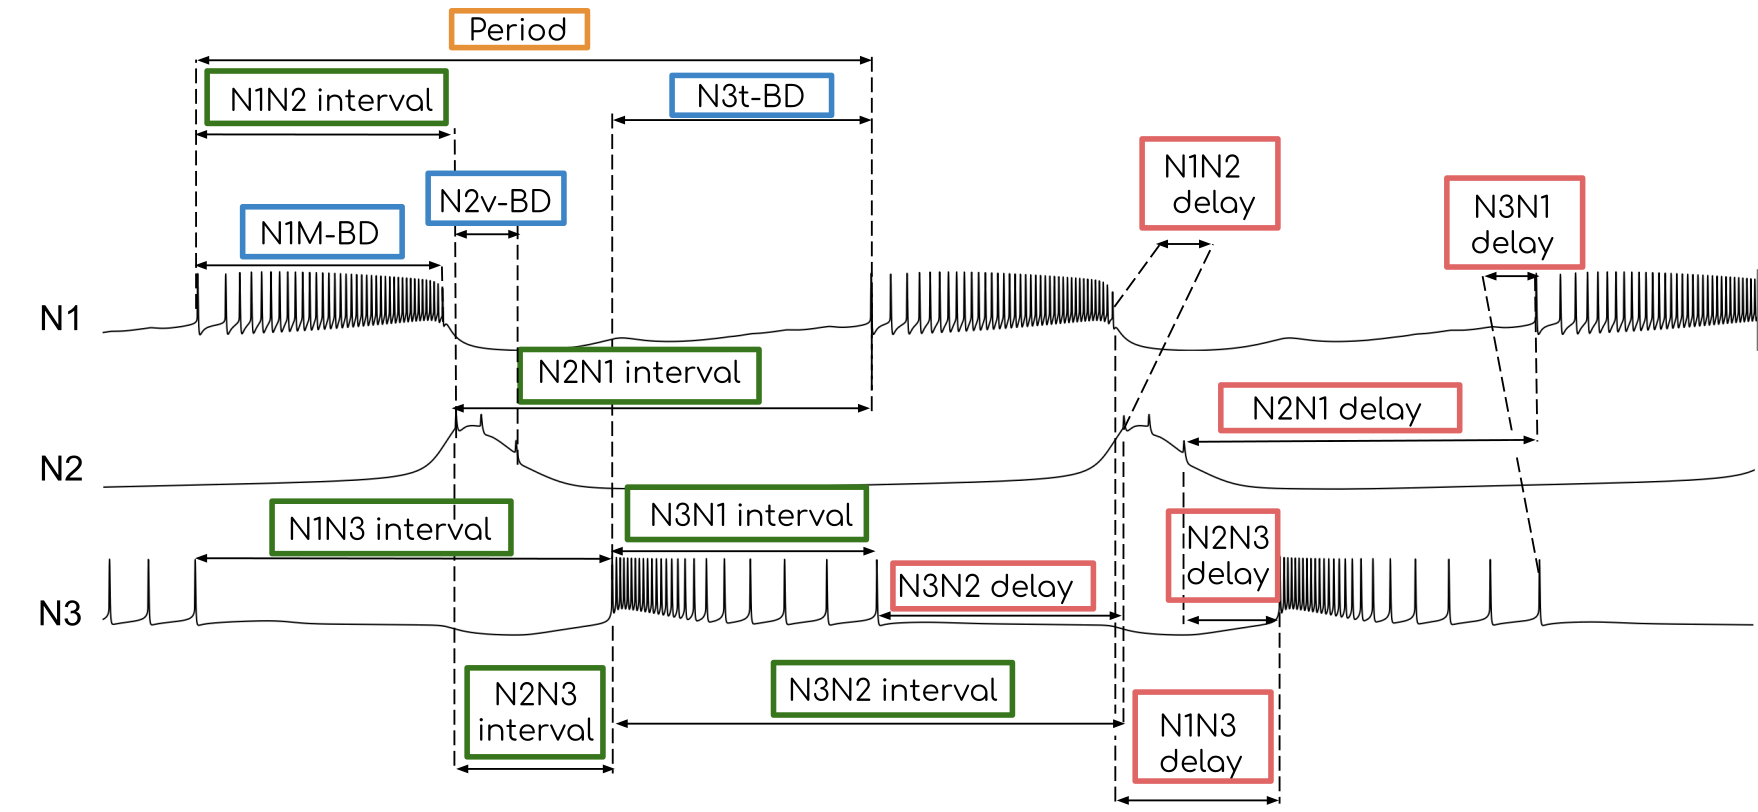
\includegraphics[width=\textwidth]{methods-paper-modelo/Intervals_figure_complete.png}
		\end{minipage}
		\centering 
		\begin{minipage}[b]{0.3\textwidth}
			\centering
			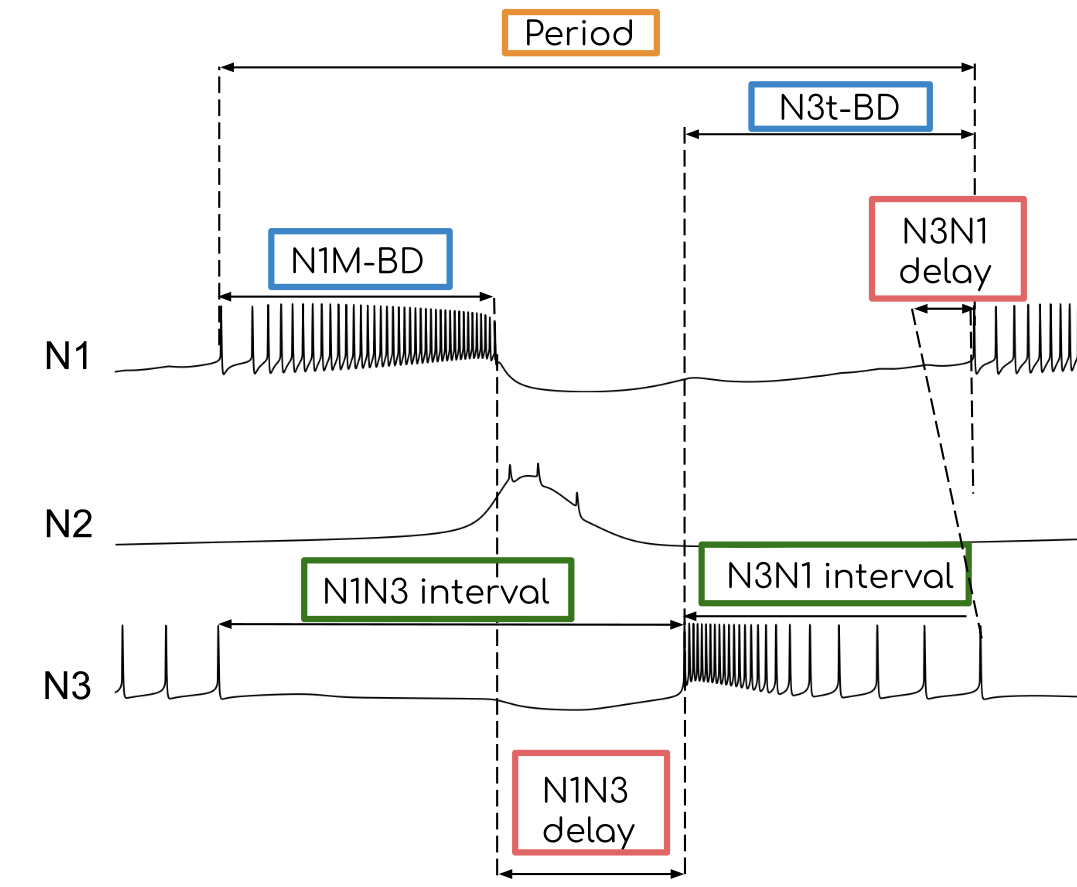
\includegraphics[width=\textwidth]{methods-paper-modelo/Intervals_figure_complete_2_phases.png}
		\end{minipage}	
	\end{minipage}\\
	\begin{minipage}[b]{0.53\textwidth}
		\centering
		\begin{minipage}[b]{\textwidth}
			\centering
			\begin{overpic}[width=\textwidth]{invariants/data/MODEL/n1m_driven/images/3phases/_durations.pdf}
				\put(0,35){\large\textbf{b)}}
			\end{overpic}
		\end{minipage}\
		\begin{minipage}[b]{\textwidth}
			\centering
			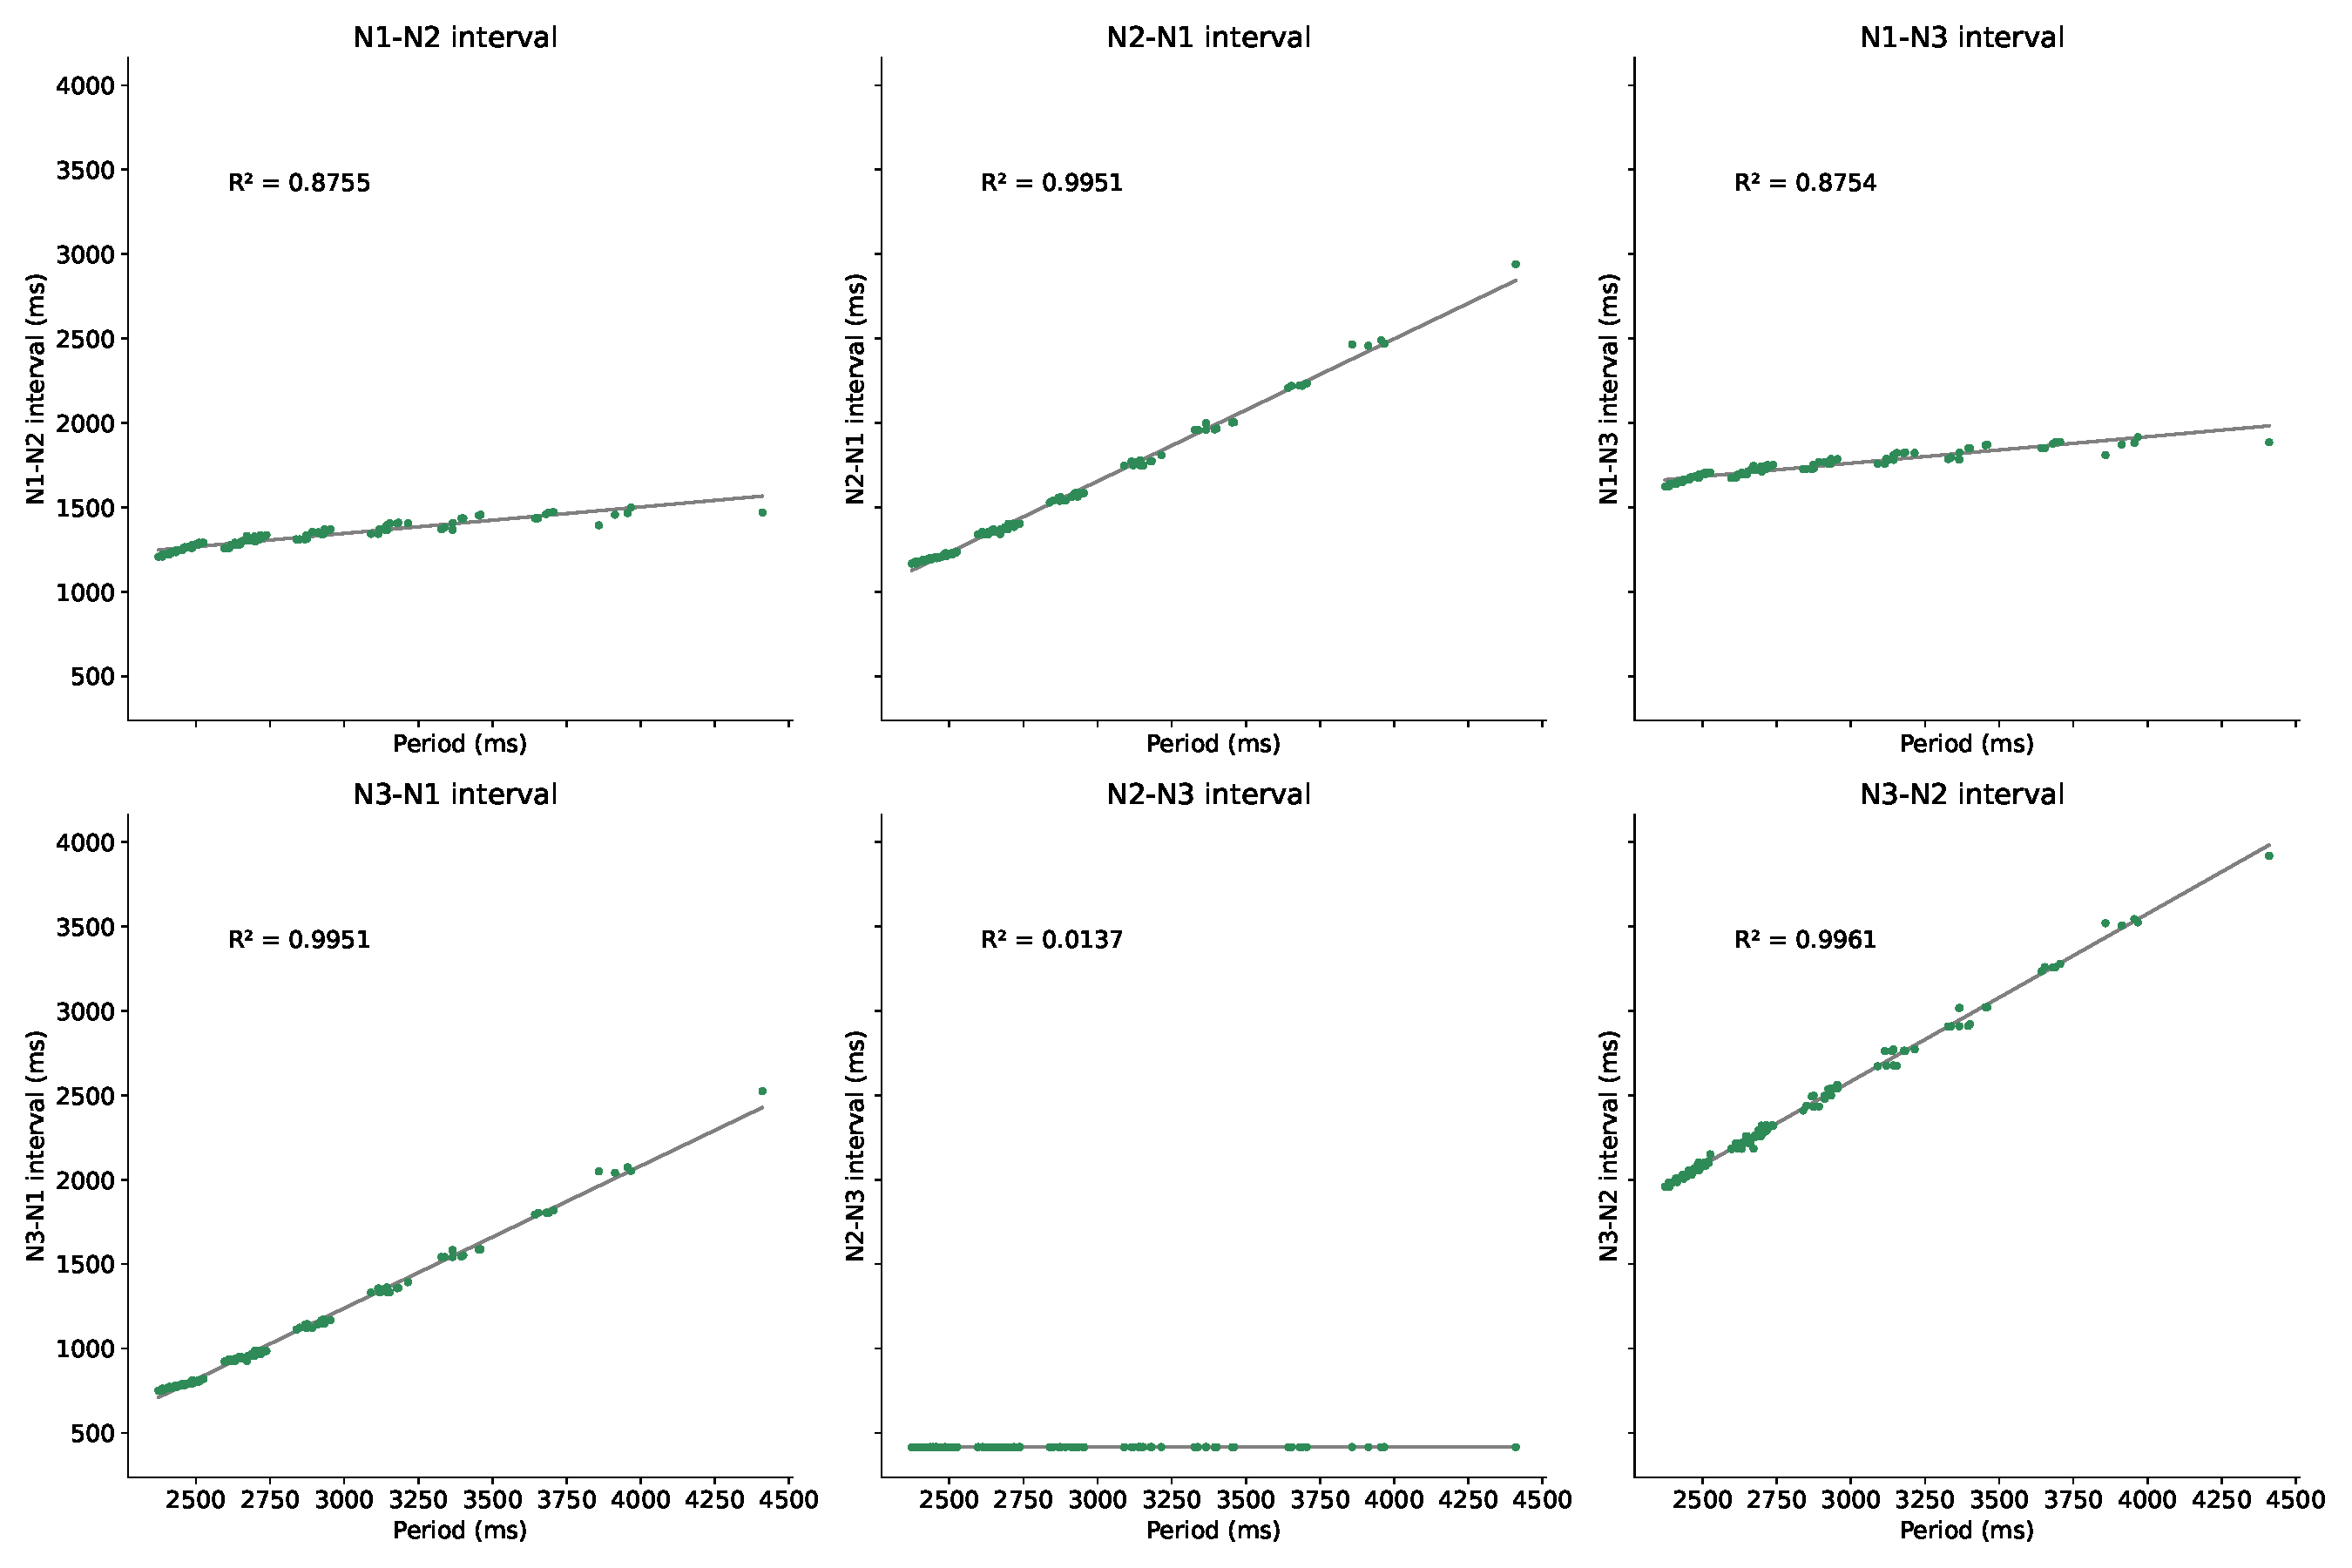
\includegraphics[width=\textwidth]{invariants/data/MODEL/n1m_driven/images/3phases/_intervals.pdf}
		\end{minipage}\
		\begin{minipage}[b]{\textwidth}
			\centering
			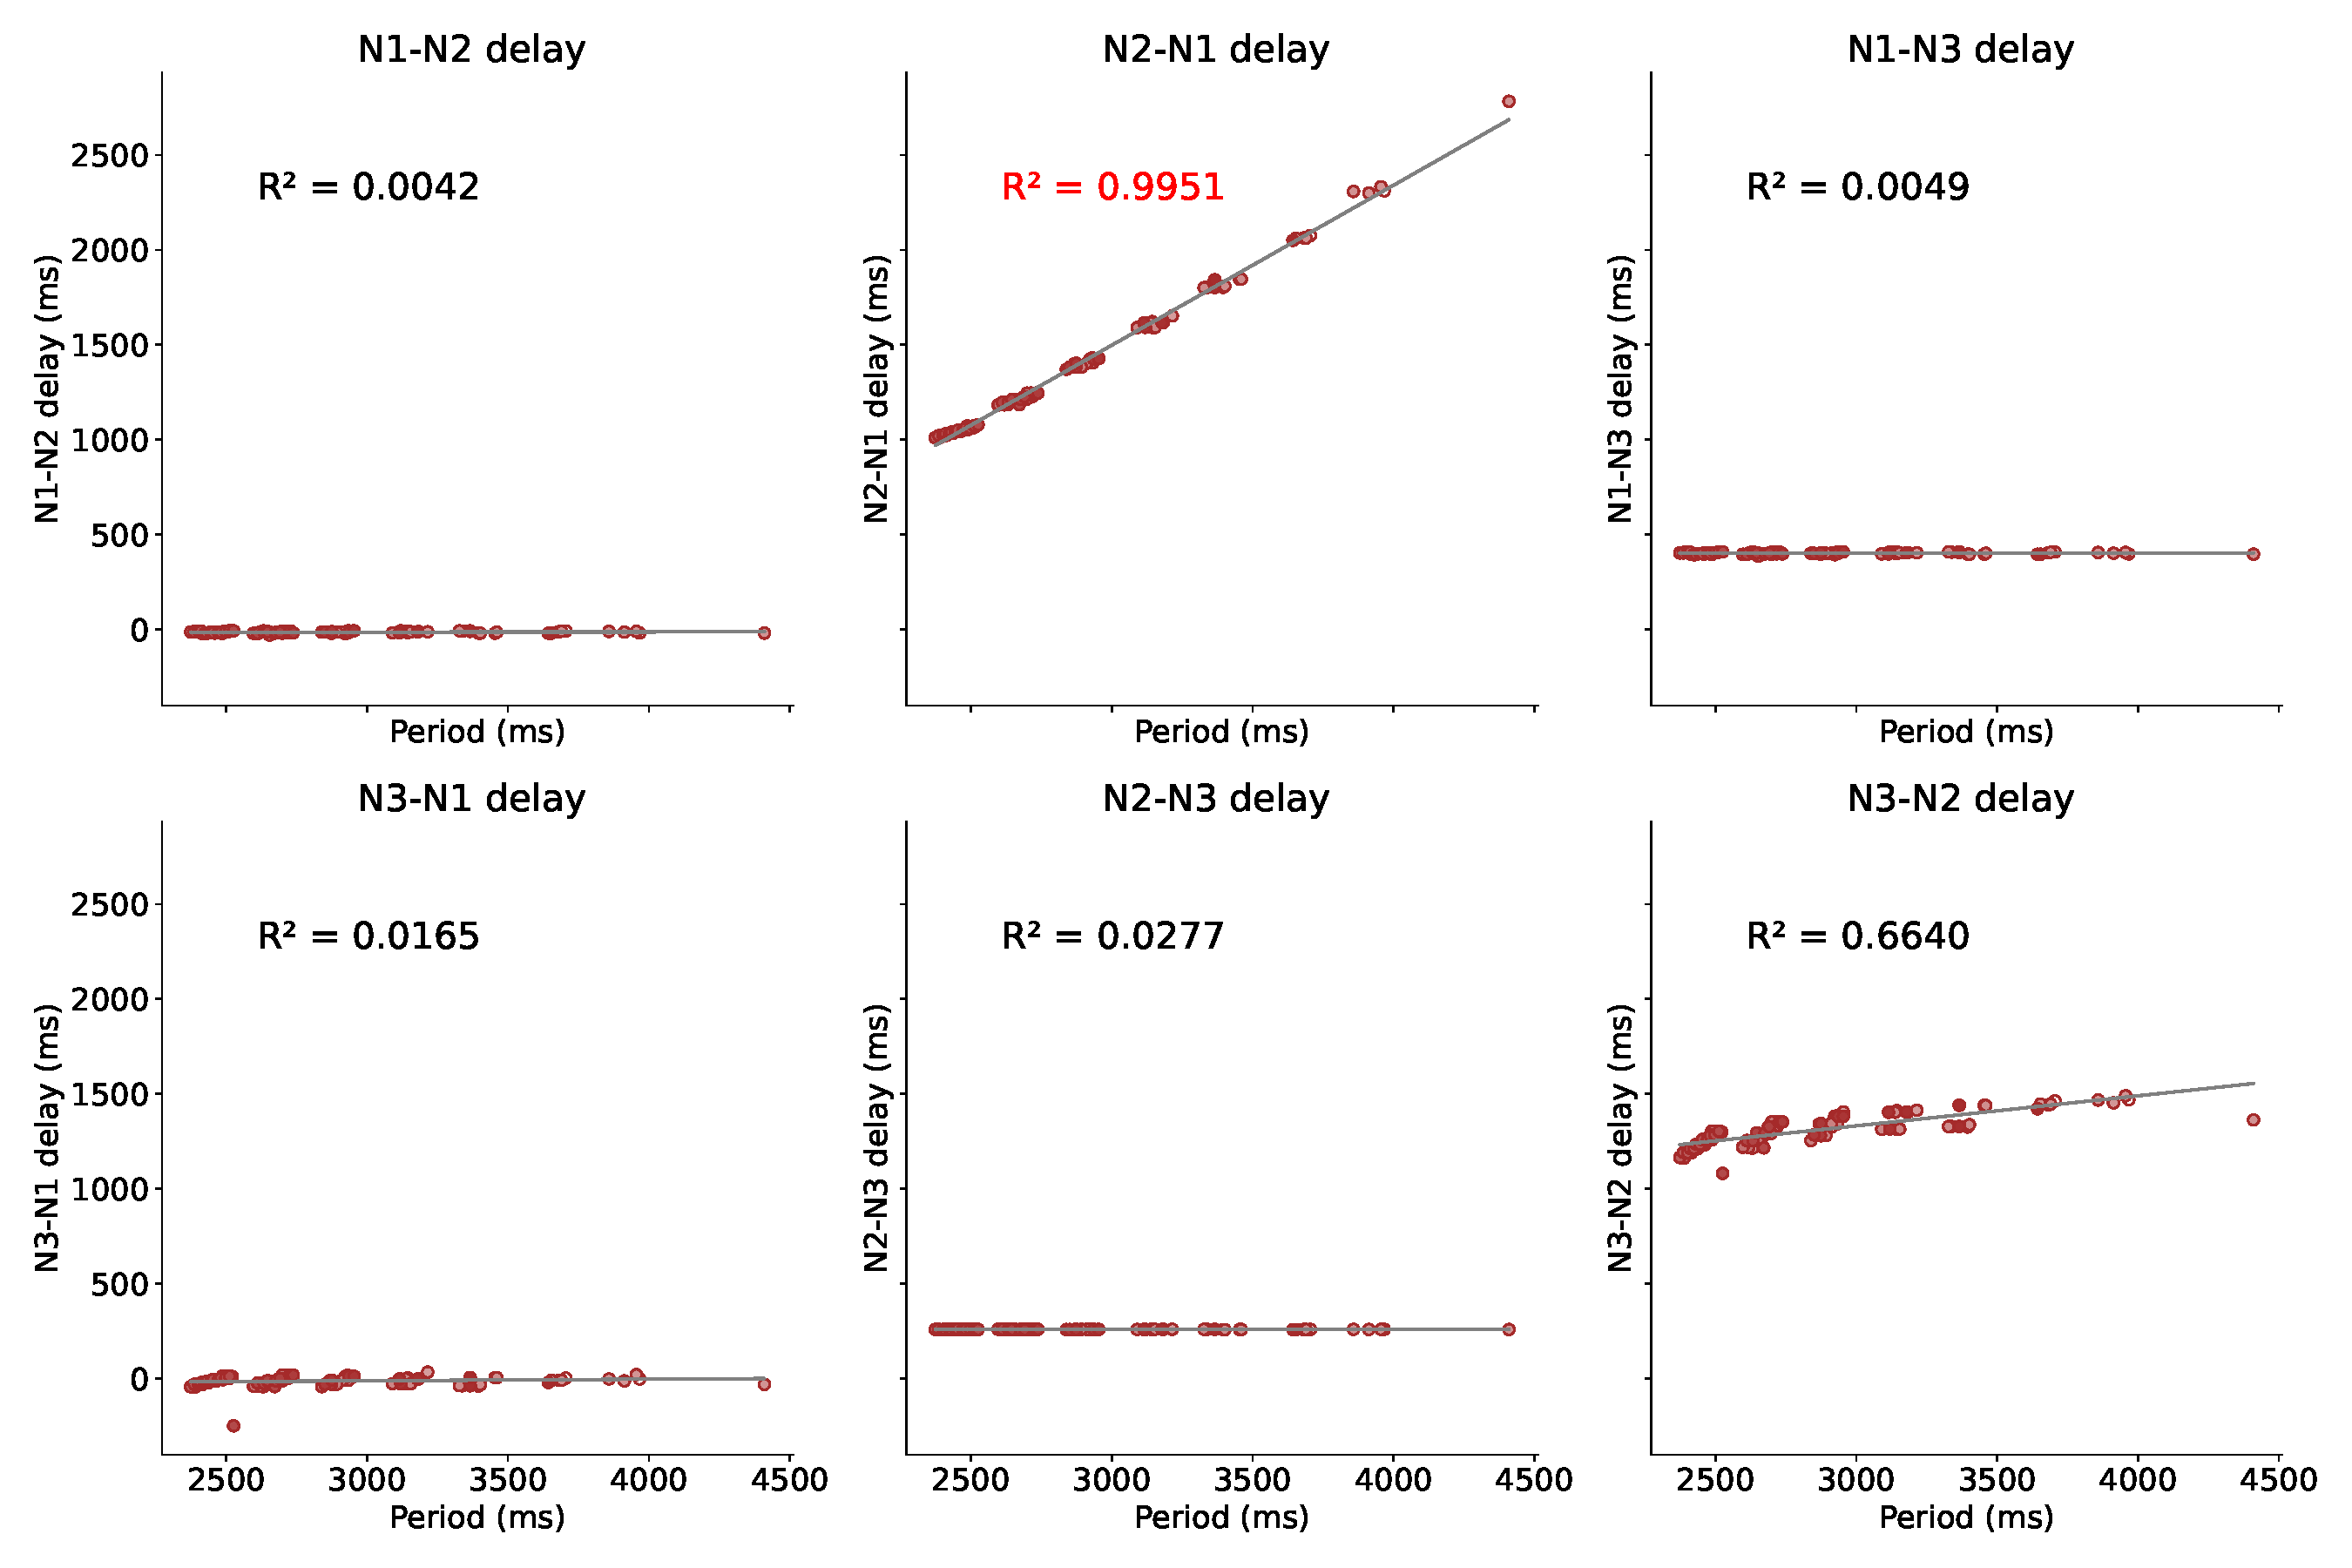
\includegraphics[width=\textwidth]{invariants/data/MODEL/n1m_driven/images/3phases/_delays.pdf}
		\end{minipage}
	\end{minipage}
	\begin{minipage}[b]{0.45\textwidth}
		\centering
		\begin{minipage}[b]{\textwidth}
			\centering
			\begin{overpic}[width=\textwidth]{invariants/data/MODEL/n1m_driven/images/2phases/_durations.pdf}
				\put(0,50){\large\textbf{c)}}
		\end{overpic}
		\end{minipage}\
		\begin{minipage}[b]{\textwidth}
			\centering
			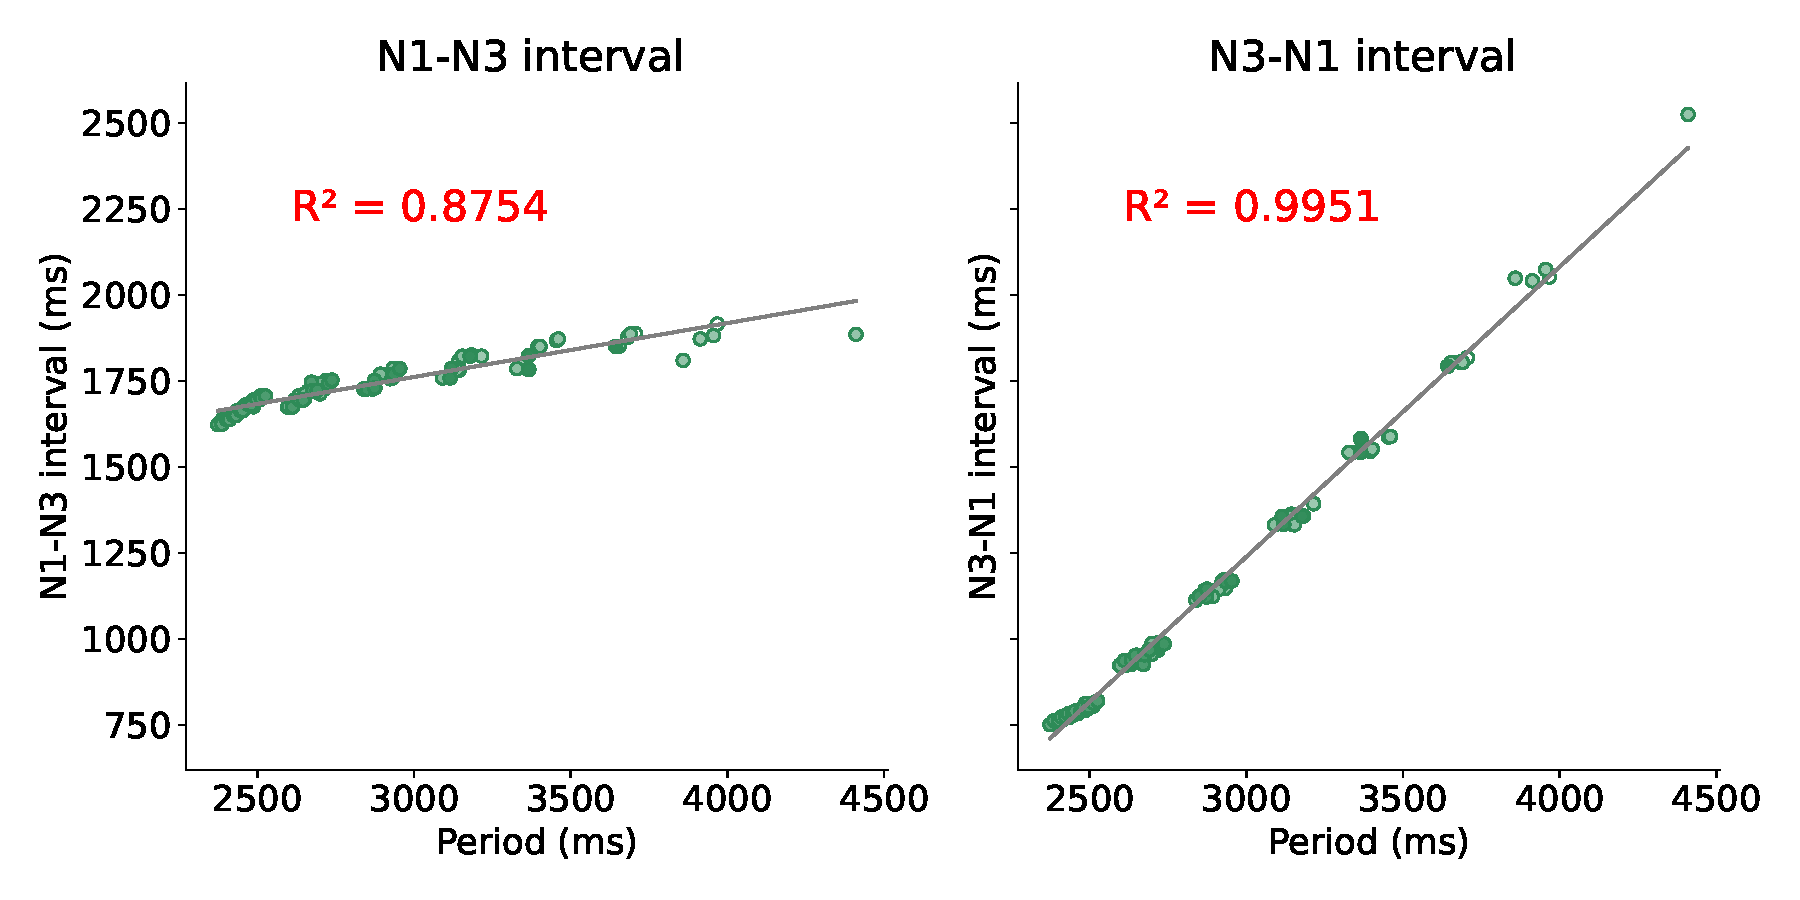
\includegraphics[width=\textwidth]{invariants/data/MODEL/n1m_driven/images/2phases/_intervals.pdf}
		\end{minipage}\
		\begin{minipage}[b]{\textwidth}
			\centering
			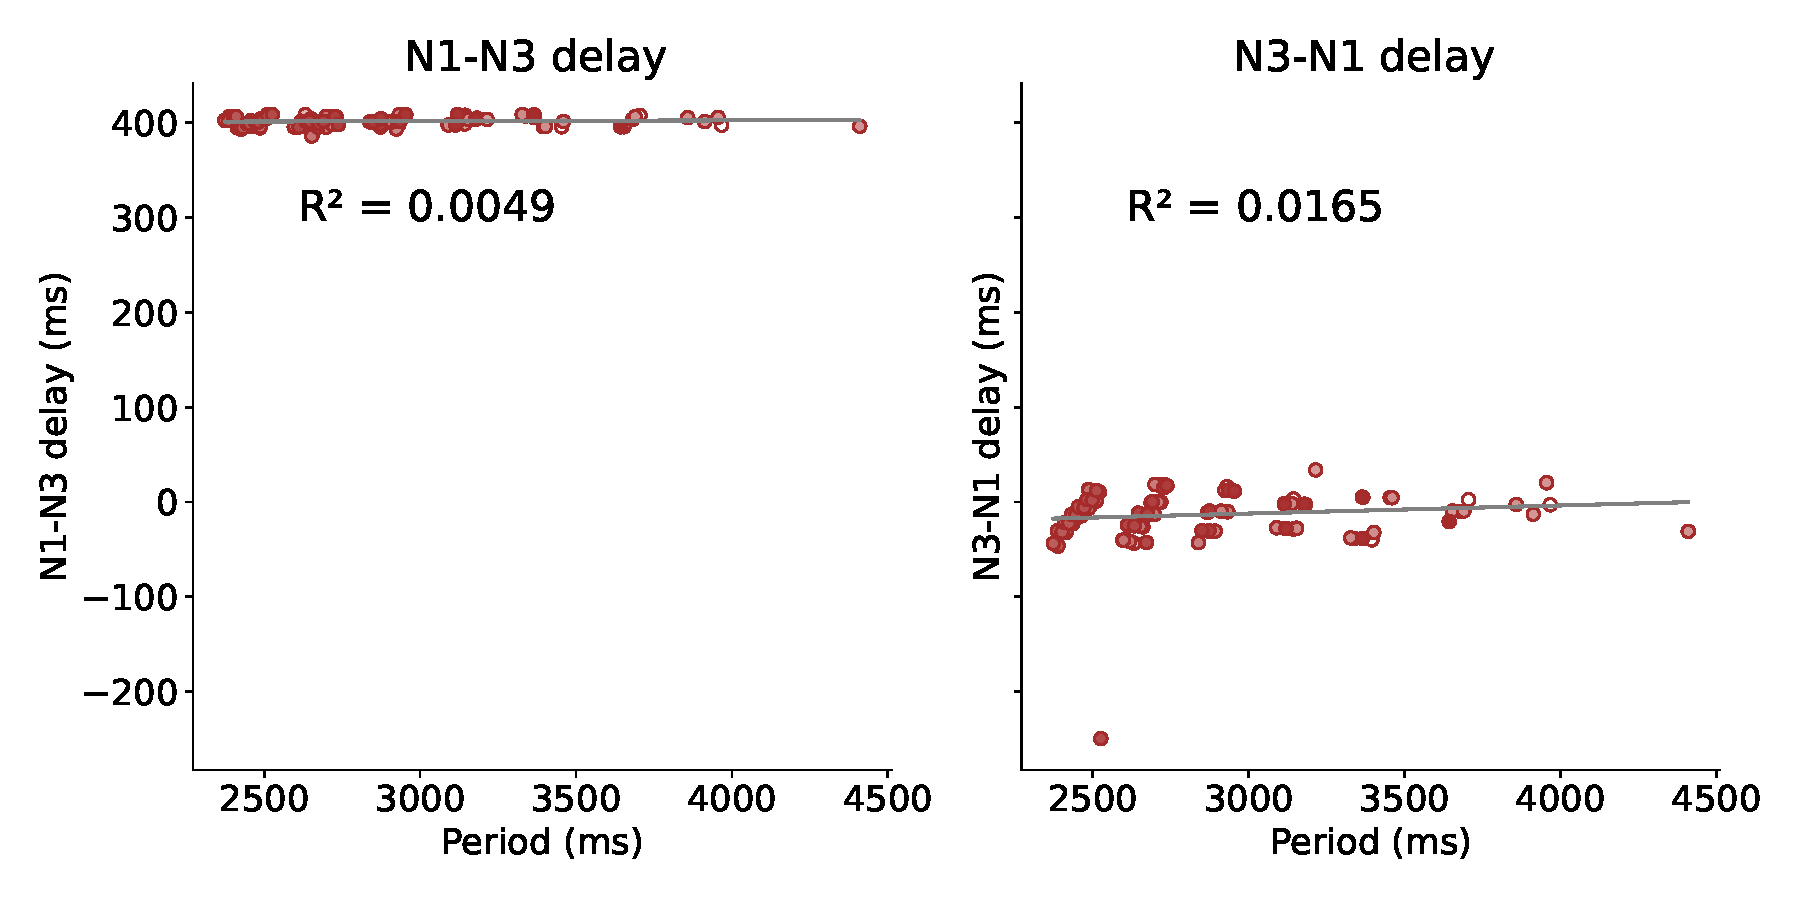
\includegraphics[width=\textwidth]{invariants/data/MODEL/n1m_driven/images/2phases/_delays.pdf}
		\end{minipage}
	
		\vspace{50pt}
	\end{minipage}
	\caption{a) Representation of the intervals for each cycle when considering three or two phases (left and right, respectively). b) Interval correlations to period for SO-driven simulation for 3 phases. First row: Burst duration. Second and third row: Two-neuron intervals. Forth and fifth row: Two-neuron delays (Data shown in Fig. \ref{fig:invariant n1m}). c) Interval correlations to period for N1M-driven simulation for 2 phases. First row: Burst duration. Second row: Two-neuron intervals. Third row: Two-neuron delays. For b) and c) the linear relationships are quantified by the $R^2$ values of the regression.}
	\label{fig:invariant n1m model 2 phases}
\end{figure}


\clearpage
\newpage
